%%%%%%%%%%%%%%%%%%%%%%%%%%%%%%%%%%%%%%%%%%%%%%%%%%%%%%%%%%%%%%%%%%%%%%%%%%%%%%%%
%%%%%%%%%%%%%%%%%%%%%%%%%%%%%%%%%%%%%%%%%%%%%%%%%%%%%%%%%%%%%%%%%%%%%%%%%%%%%%%%
%%%%%%%%%%%%%%%%%%%%%%%%%%%%%%%%%%%%%%%%%%%%%%%%%%%%%%%%%%%%%%%%%%%%%%%%%%%%%%%%
\chapter{Condiciones experimentales}
\label{cha:detector}
%%%%%%%%%%%%%%%%%%%%%%%%%%%%%%%%%%%%%%%%%%%%%%%%%%%%%%%%%%%%%%%%%%%%%%%%%%%%%%%%
%%%%%%%%%%%%%%%%%%%%%%%%%%%%%%%%%%%%%%%%%%%%%%%%%%%%%%%%%%%%%%%%%%%%%%%%%%%%%%%%
%%%%%%%%%%%%%%%%%%%%%%%%%%%%%%%%%%%%%%%%%%%%%%%%%%%%%%%%%%%%%%%%%%%%%%%%%%%%%%%%

\todo{this chapter is not fully corrected yet}

\color{vero}
En 1954 se funda el Laboratorio Europeo para la Física de Partículas, CERN\footnote{Las siglas provienen del previo acrónimo francés de \emph{Conseil Européen pour la Recherche Nucléaire}, aunque en la actualidad el nombre del centro es \emph{Organisation européenne pour la recherche nucléaire}.}, internacionalizando la investigación en este campo, haciéndola más transparente y segura.
%
Con el paso del tiempo, se pudieron alcanzar cada vez energías mayores en el acelerador principal.%y el \cern se fue centrando en el estudio de la física de partículas y dejando en una fracción pequeña a la física nuclear.
\color{norm}

\begin{table}[H]
\centering
\begin{tabular}{l|p{7cm}r}
1957 -- 1990 & \textit{Synchrocyclotron} & $600$ MeV \\ 
 & Primer acelerador del CERN. \\
1959    --      &  \textit{Proton Synchrotron} & $26$ GeV\\ 
& Se continúa usando en la actualidad como pre--acelerador.\\
1971 -- 1984 & \textit{Intersecting Storage Rings} & $62$ GeV\\
     & Primer colisionador de hadrones del mundo.\\     
1976 -- & \textit{Super Proton Synchrotron} & $450$ GeV\\
& En él se descubrieron las corrientes neutras, y se continúa usando en la actualidad como pre--acelerador.\\
1984 -- 2000 & \textit{Large Electron--Positron}\\
& Confirmó la existencia de 3 familias de fermiones y el \stdmod con muy buena precisión.\\
2008 --      & \textit{Large Hadron Collider} & $7$ TeV \\
& Es el mayor acelerador de protones del mundo, y en él se ha observado por primera vez el bosón de Higgs.
\end{tabular}
\caption{Cronología de los principales aceleradores en el \cern.}
\end{table}

\vspace*{\fill}

\begin{figure}[H]
\centering
\subfloat[Proyección del \lhc sobre la superficie terrestre, junto con las partes principales \cite{lhcpathearth}. \label{fig_lhcB}]{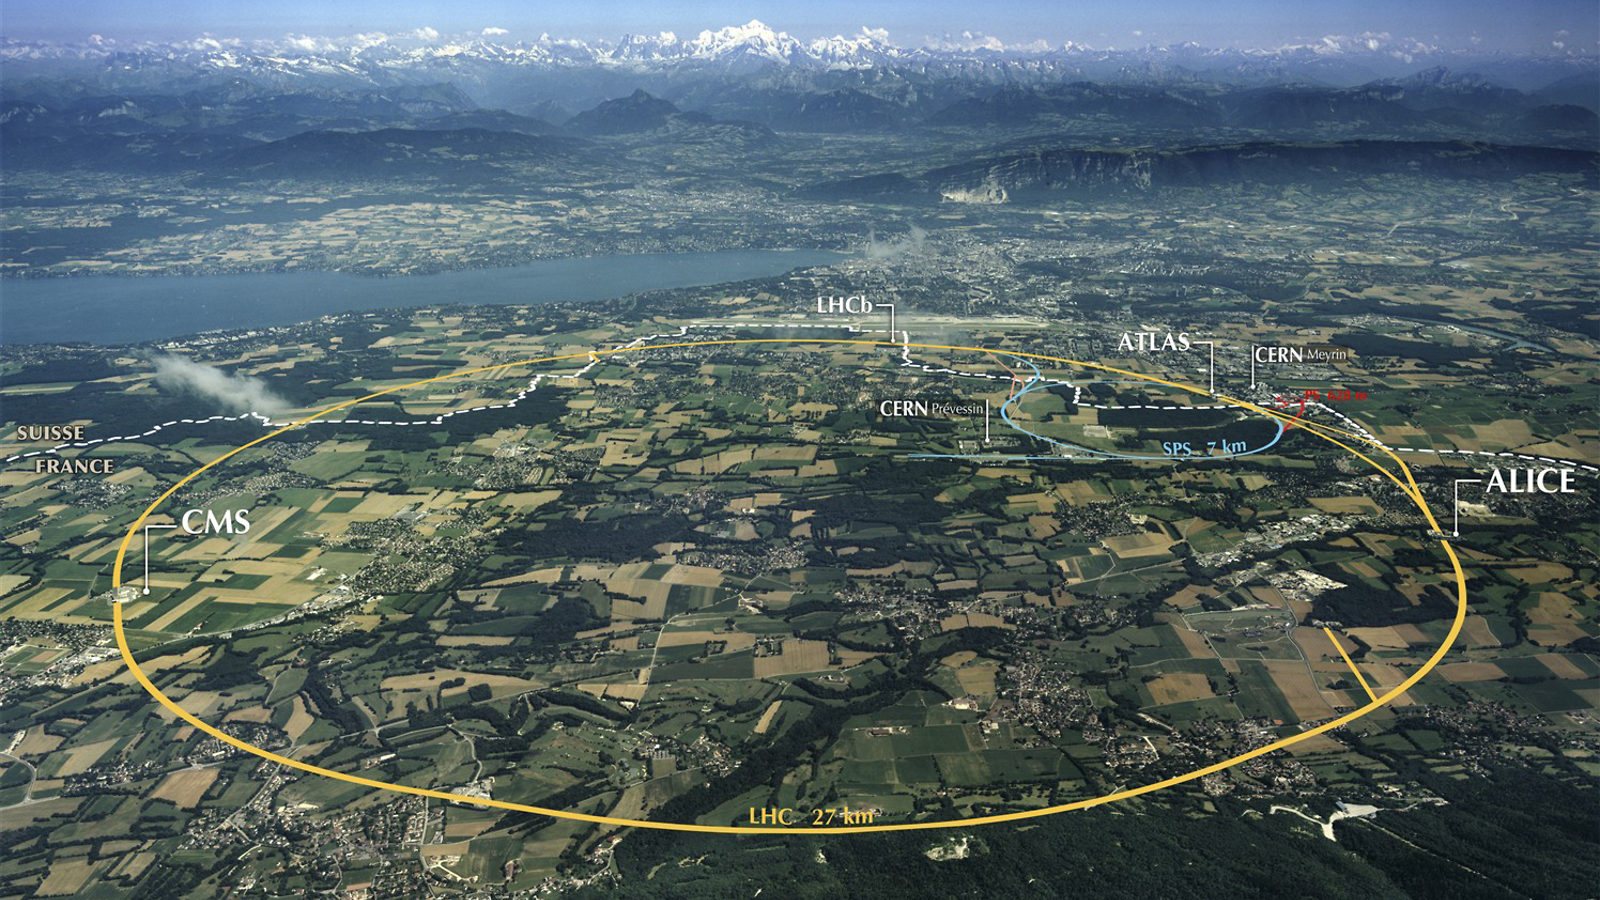
\includegraphics[width=\textwidth]{LHCearth}} \\ \vfill
\subfloat[Cadena de aceleradores con la que se inyectan protones al \lhc. \label{fig_lhcA}]{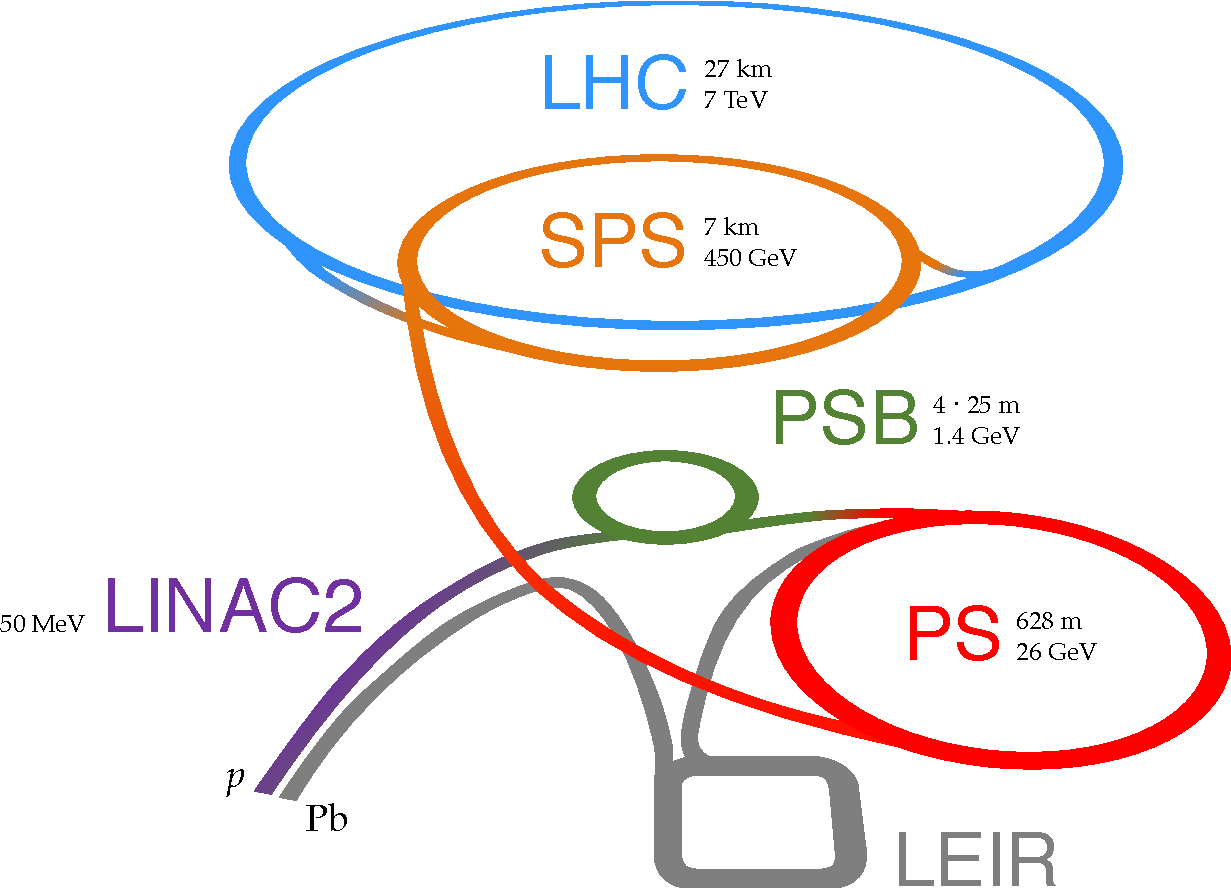
\includegraphics[width=\textwidth]{LHCChain}}  \vfill
\caption{Disposición de los elementos principales del \lhc.} \label{fig_lhc}
\end{figure}

\vspace*{\fill}

\newpage


%%%%%%%%%%%%%%%%%%%%%%%%%%%%%%%%%%%%%%%%%%%%%%%%%%%%%%%%%%%%%%%%%%%%%%%%%%%%%%%%
\section{El CERN y su acelerador \lhc} %%%%%%%%%%%%%%%%%%%%%%%%%%%%%%%%%%%%%%%%%%%%%%%%%%%%%%%%%


El LHC es un acelerador circular de 27 km de longitud diseñado para producir colisiones $p-p$ a una energía máxima en el centro de masa de $\sqrt{s} = 14 \, \mathrm{TeV}$, permitiendo por tanto estudiar la escala de energías de $10^{12}$ eV y buscar nueva física. \color{vero} Desde 2008 opera en la misma obra civil que lo hacía LEP, \color{norm} soterrado a unos 150 metros de profundidad en la frontera franco-suiza, cerca de Ginebra como se ve en la Figura \ref{fig_lhcA}.

Los protones se extraen de fuentes de iones, como el duoplasmatrón, introduciendo gas hidrógeno,
y se van acelerando en una sucesión de  pre--aceleradores: LINAC, PSB, PS y  SPS, hasta finalmente llegar al LHC donde se alcanzan los $7 \, \mathrm{TeV}$ por haz (\emph{vid.} Figura \ref{fig_lhcA}).
%
Estos haces contienen $1.15 \times  10^{11}$ protones y se hacen cruzar con una frecuencia de $40$ MHz, dando el acelerador una luminosidad máxima de $10^{34} \, \mathrm{cm^{-2}s^{-1}}$.


A estas energías tan altas, para mantener a las dos corrientes de protones circulando a casi la velocidad de la luz y en órbitas contrarias, se necesitan fuertes campos magnéticos ($8.33 \, \mathrm{T}$ a $7 \, \mathrm{TeV}$), que se logran mediante potentes imanes superconductores refrigerados mediante helio super--fluido a  temperaturas de aproximadamente $1.9 \, \text{K}$. Para ello se  emplea un único crióstato con un flujo magnético circulando en sentido opuesto para cada corriente de protones.
 






La colisión de los dos haces tiene lugar en cuatro puntos  concretos del túnel, donde se hacen coincidir las trayectorias de ambos. 
Es en esos puntos dónde se sitúan los cuatro principales\footnote{Existen otros experimentos como TOTEM, que mide la secciones eficaces elásticas e inelásticas de las colisiones $pp$ ayudando al monitoreo de la luminosidad de CMS; o LHCf, que estudia a través los neutrones y fotones producidos a bajo ángulo en ATLAS los fenómenos de rayos cósmicos.} experimentos del LHC:

\begin{itemize}
 \item ALICE: Se dedica al estudio del Plasma de cuark y Gluones (\textit{cuark--Gluon Plasma}, QGP), un nuevo estado de agregación de la materia de extrema densidad y que se produce tras colisiones con iones pesados, para lo que se hacen circular iones Pb, en vez de protones.
 \item ATLAS: Creado para buscar el bosón de Higgs, es un detector de propósito general centrado en el estudio de los cuarks t y b; diseñado para la detección de nuevas partículas pesadas en su capa de masa, buscando nueva física, así como evidencias de partículas de SUSY.
 \item CMS: Concebido para verificar de un modo distinto los resultados de ATLAS, es también un detector de propósito general con un programa de física similar.
 \item \lhcb: Es un detector especializado en medidas de precisión en violación CP, lo hace estudiando desintegraciones de los cuarks b y c, teniendo como objetivo final entender mejor la asimetría bariónica del Universo, cuyo origen no se comprende en el \stdmod.
\end{itemize}

\color{vero}
Pueden verse representaciones de los cuatro detectores en la Figura \ref{fig_lhcdetect}. Cabe resaltar que el hito más grande, hasta la fecha, de ATLAS y CMS es el descubrimiento del bosón de Higgs en 2012; mientras que para \lhcb sus hitos son el descubrimiento de la desintegración ultra-rara $\Bs \rightarrow \muon \antimuon$, las medidas más precisas en las fases $\gamma$ y $\phis$, y el primer descubrimiento de estados de pentacuark.


\begin{figure}[H]
\subfloat[Detector ALICE \cite{alicedetector}.]{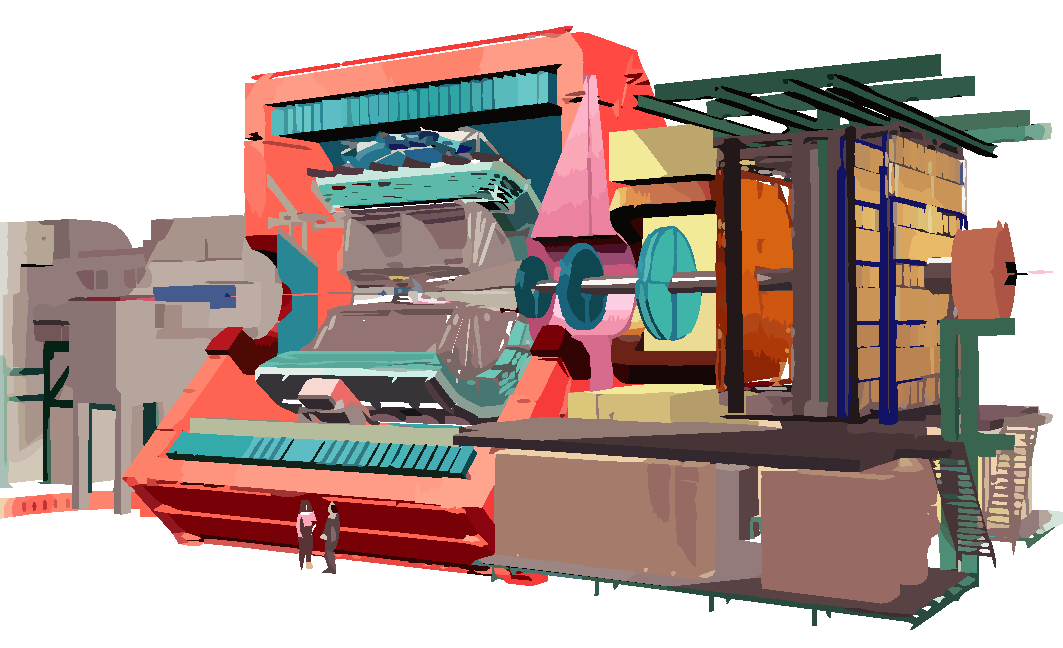
\includegraphics[width=0.48\textwidth]{ALICE.pdf}} \hfill
\subfloat[Detector ATLAS \cite{atlasdetector}.]{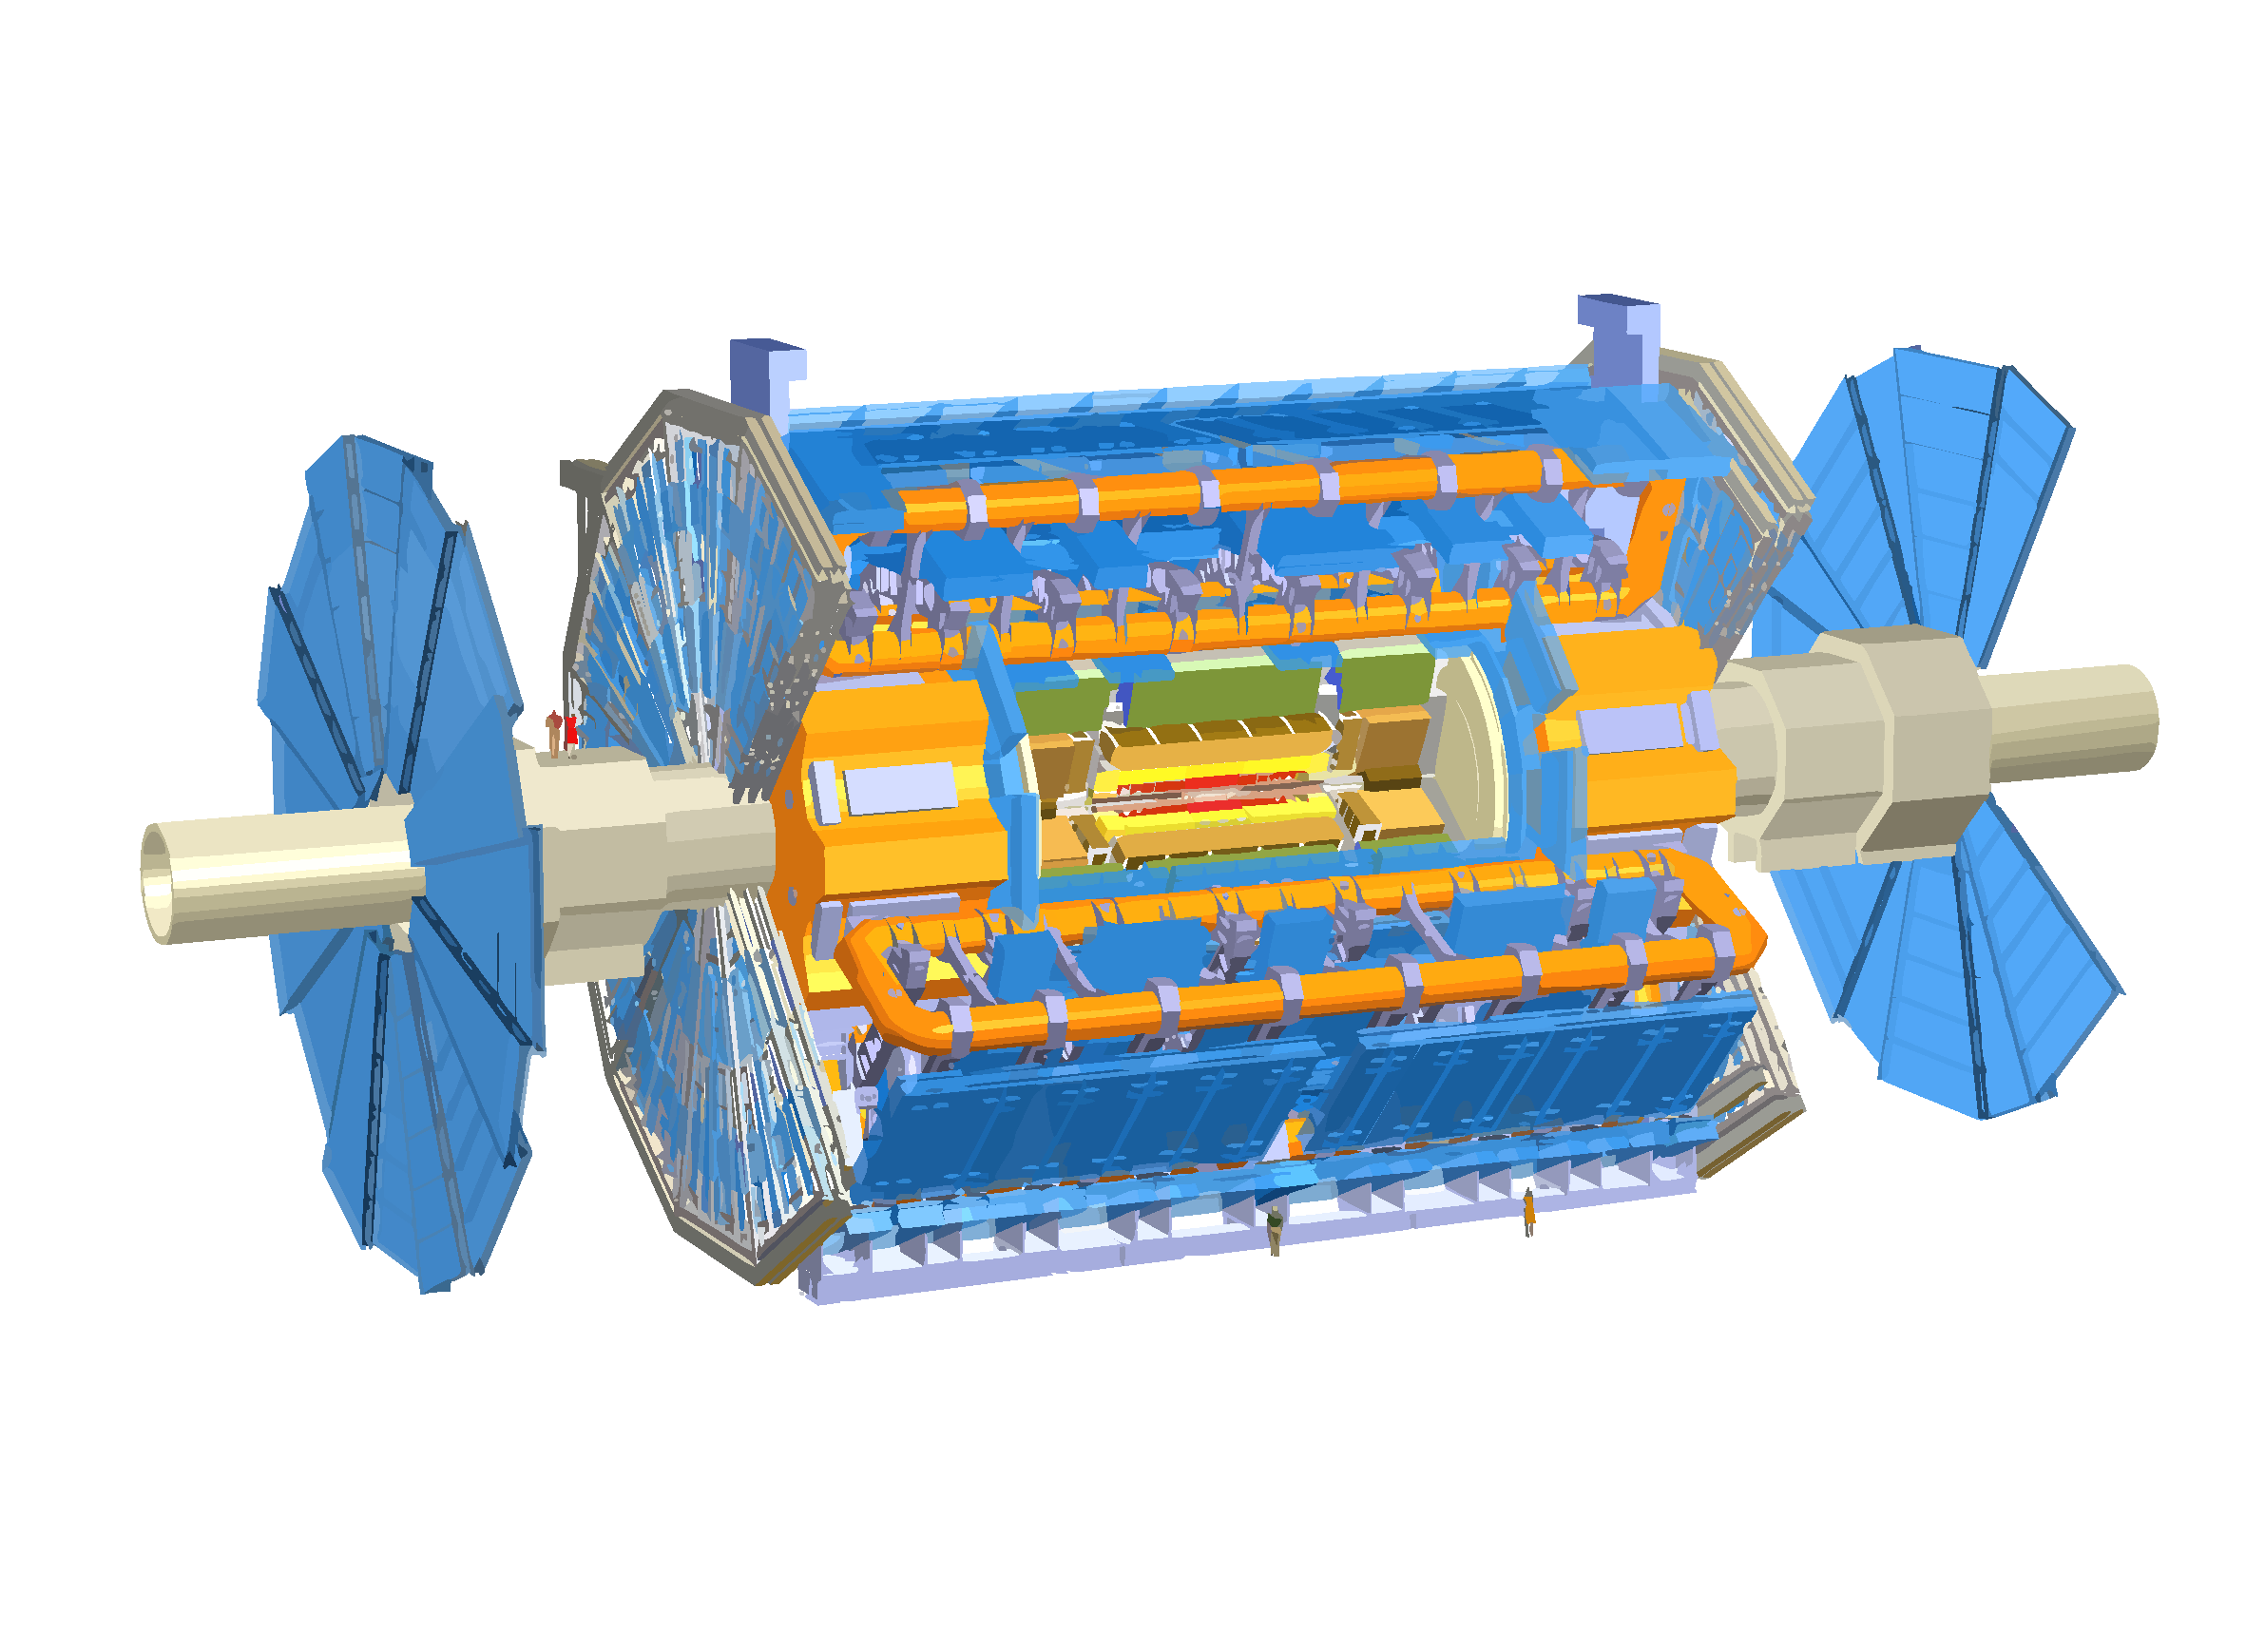
\includegraphics[width=0.48\textwidth]{ATLAS.pdf}} \hfill
%
\subfloat[Detector CMS \cite{cmsdetector}.]{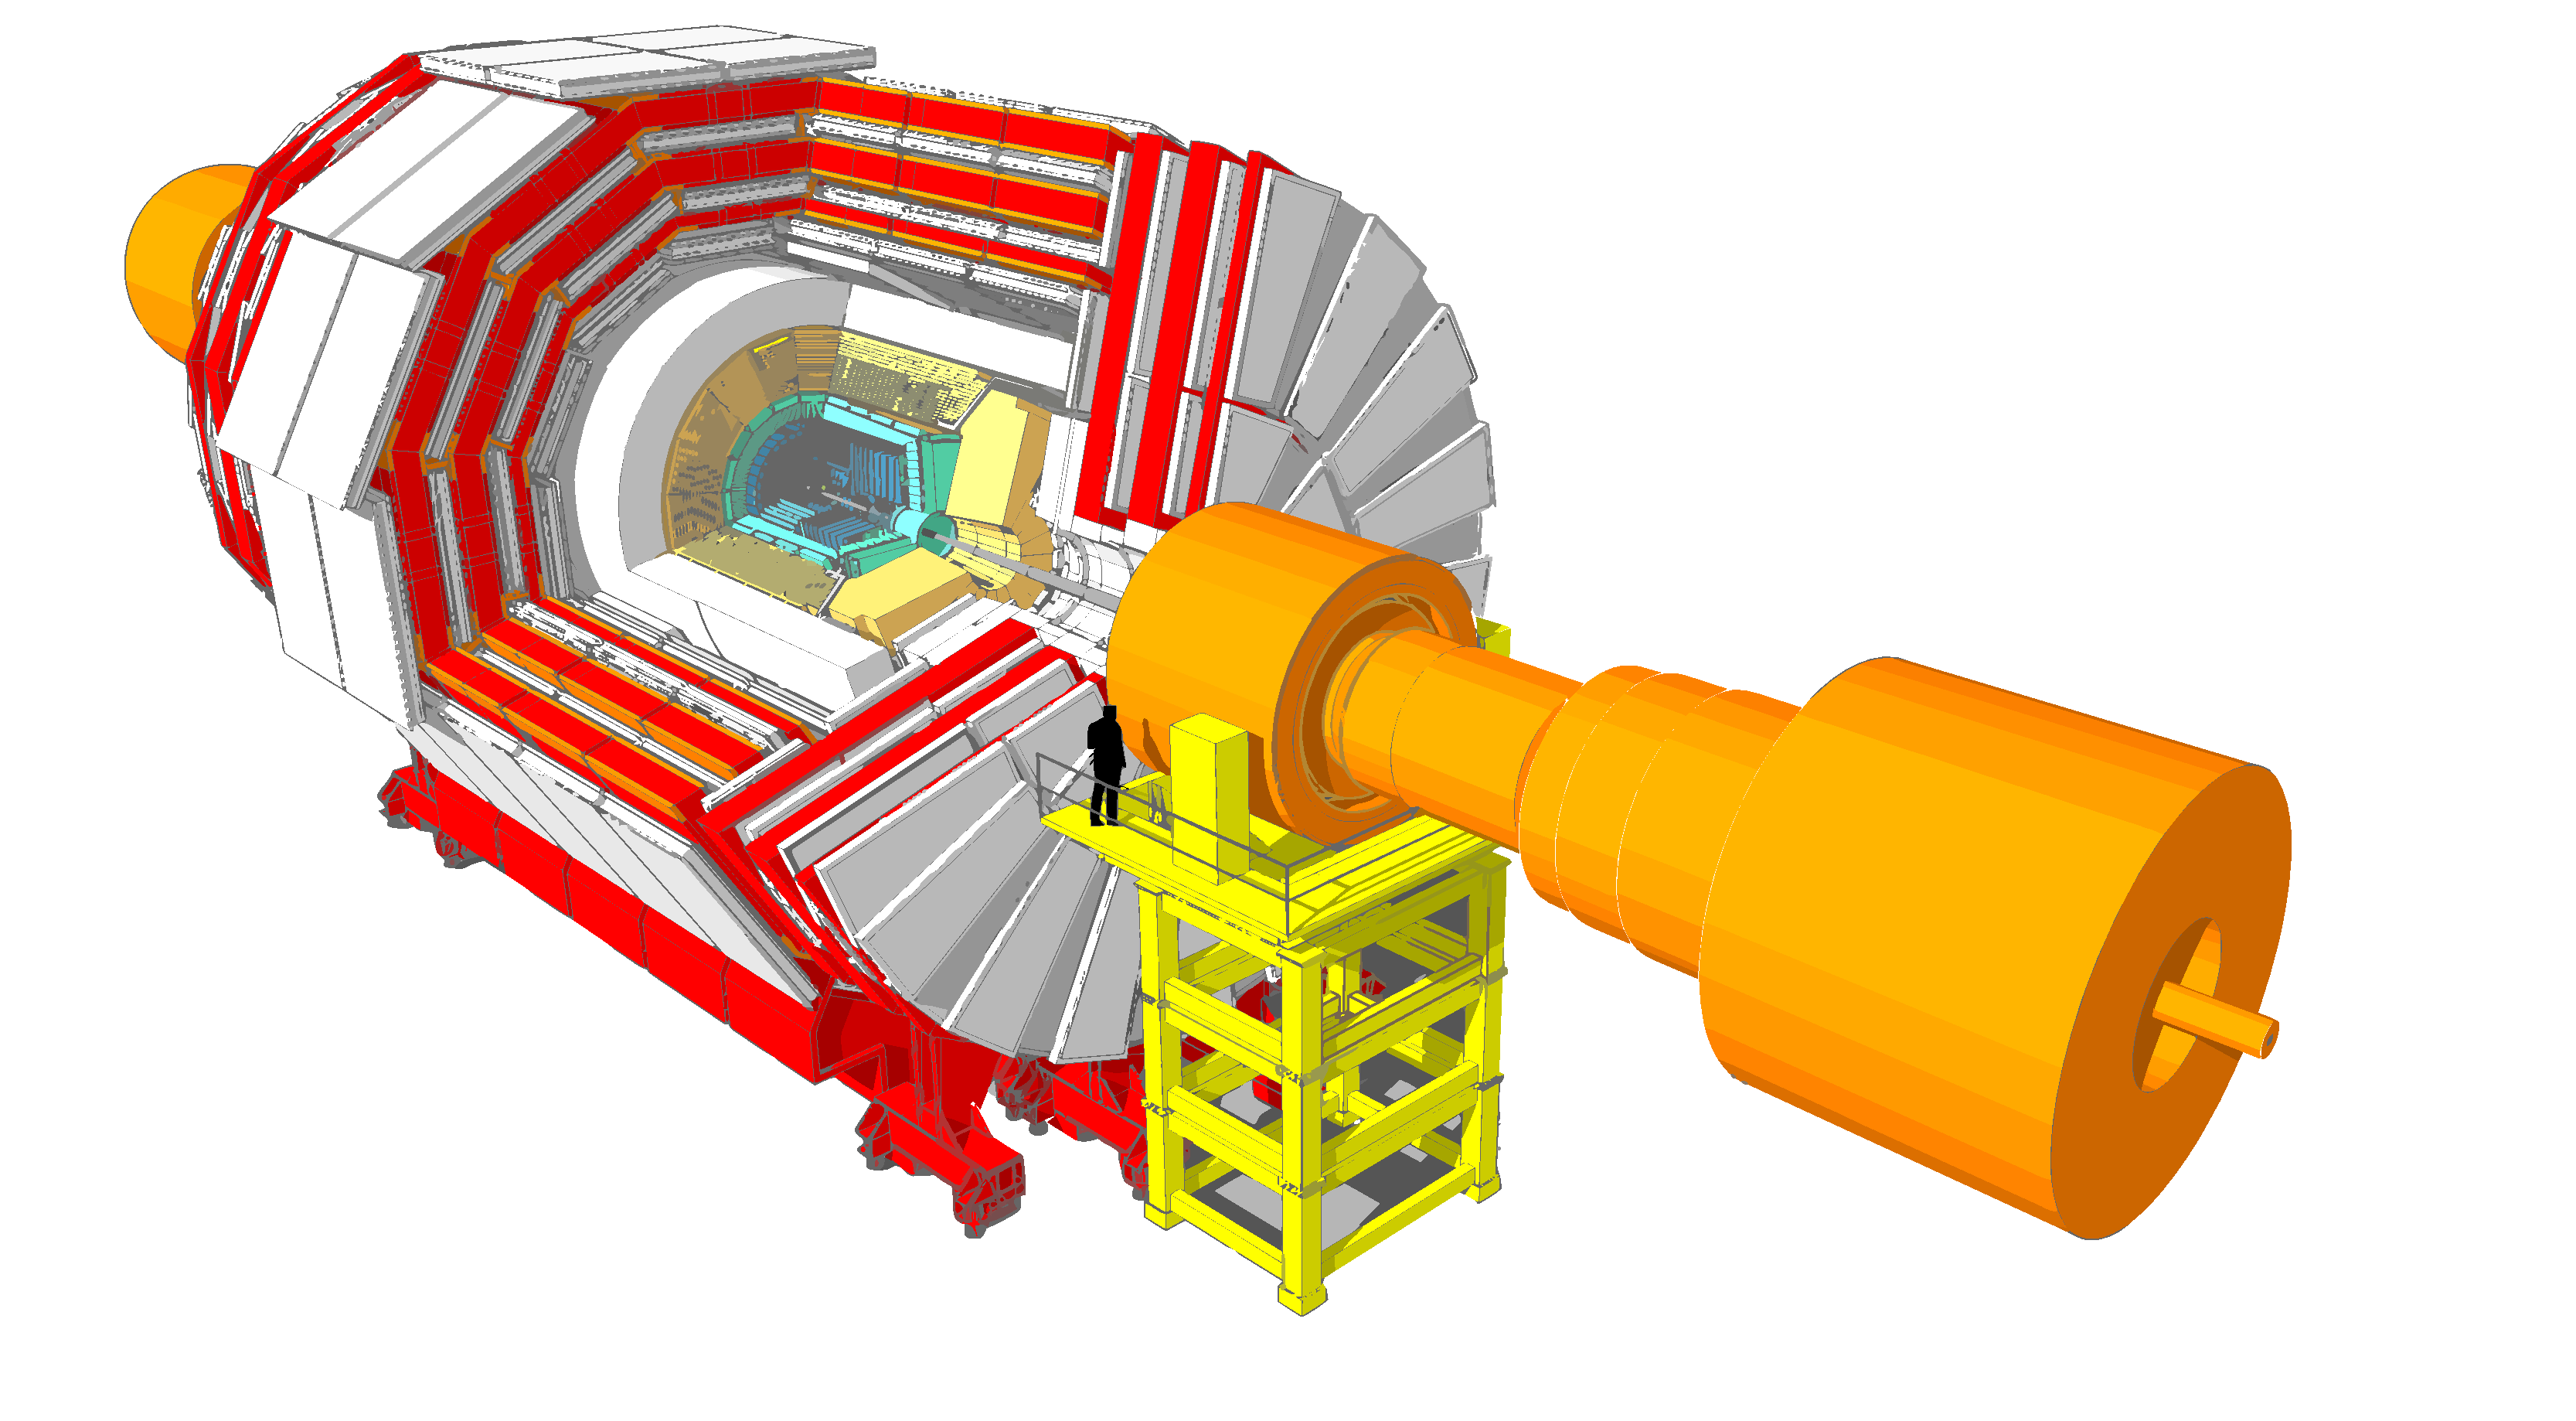
\includegraphics[width=0.48\textwidth]{CMS.pdf}} \hfill
\subfloat[Detector \lhcb \cite{lhcbdetector}.]{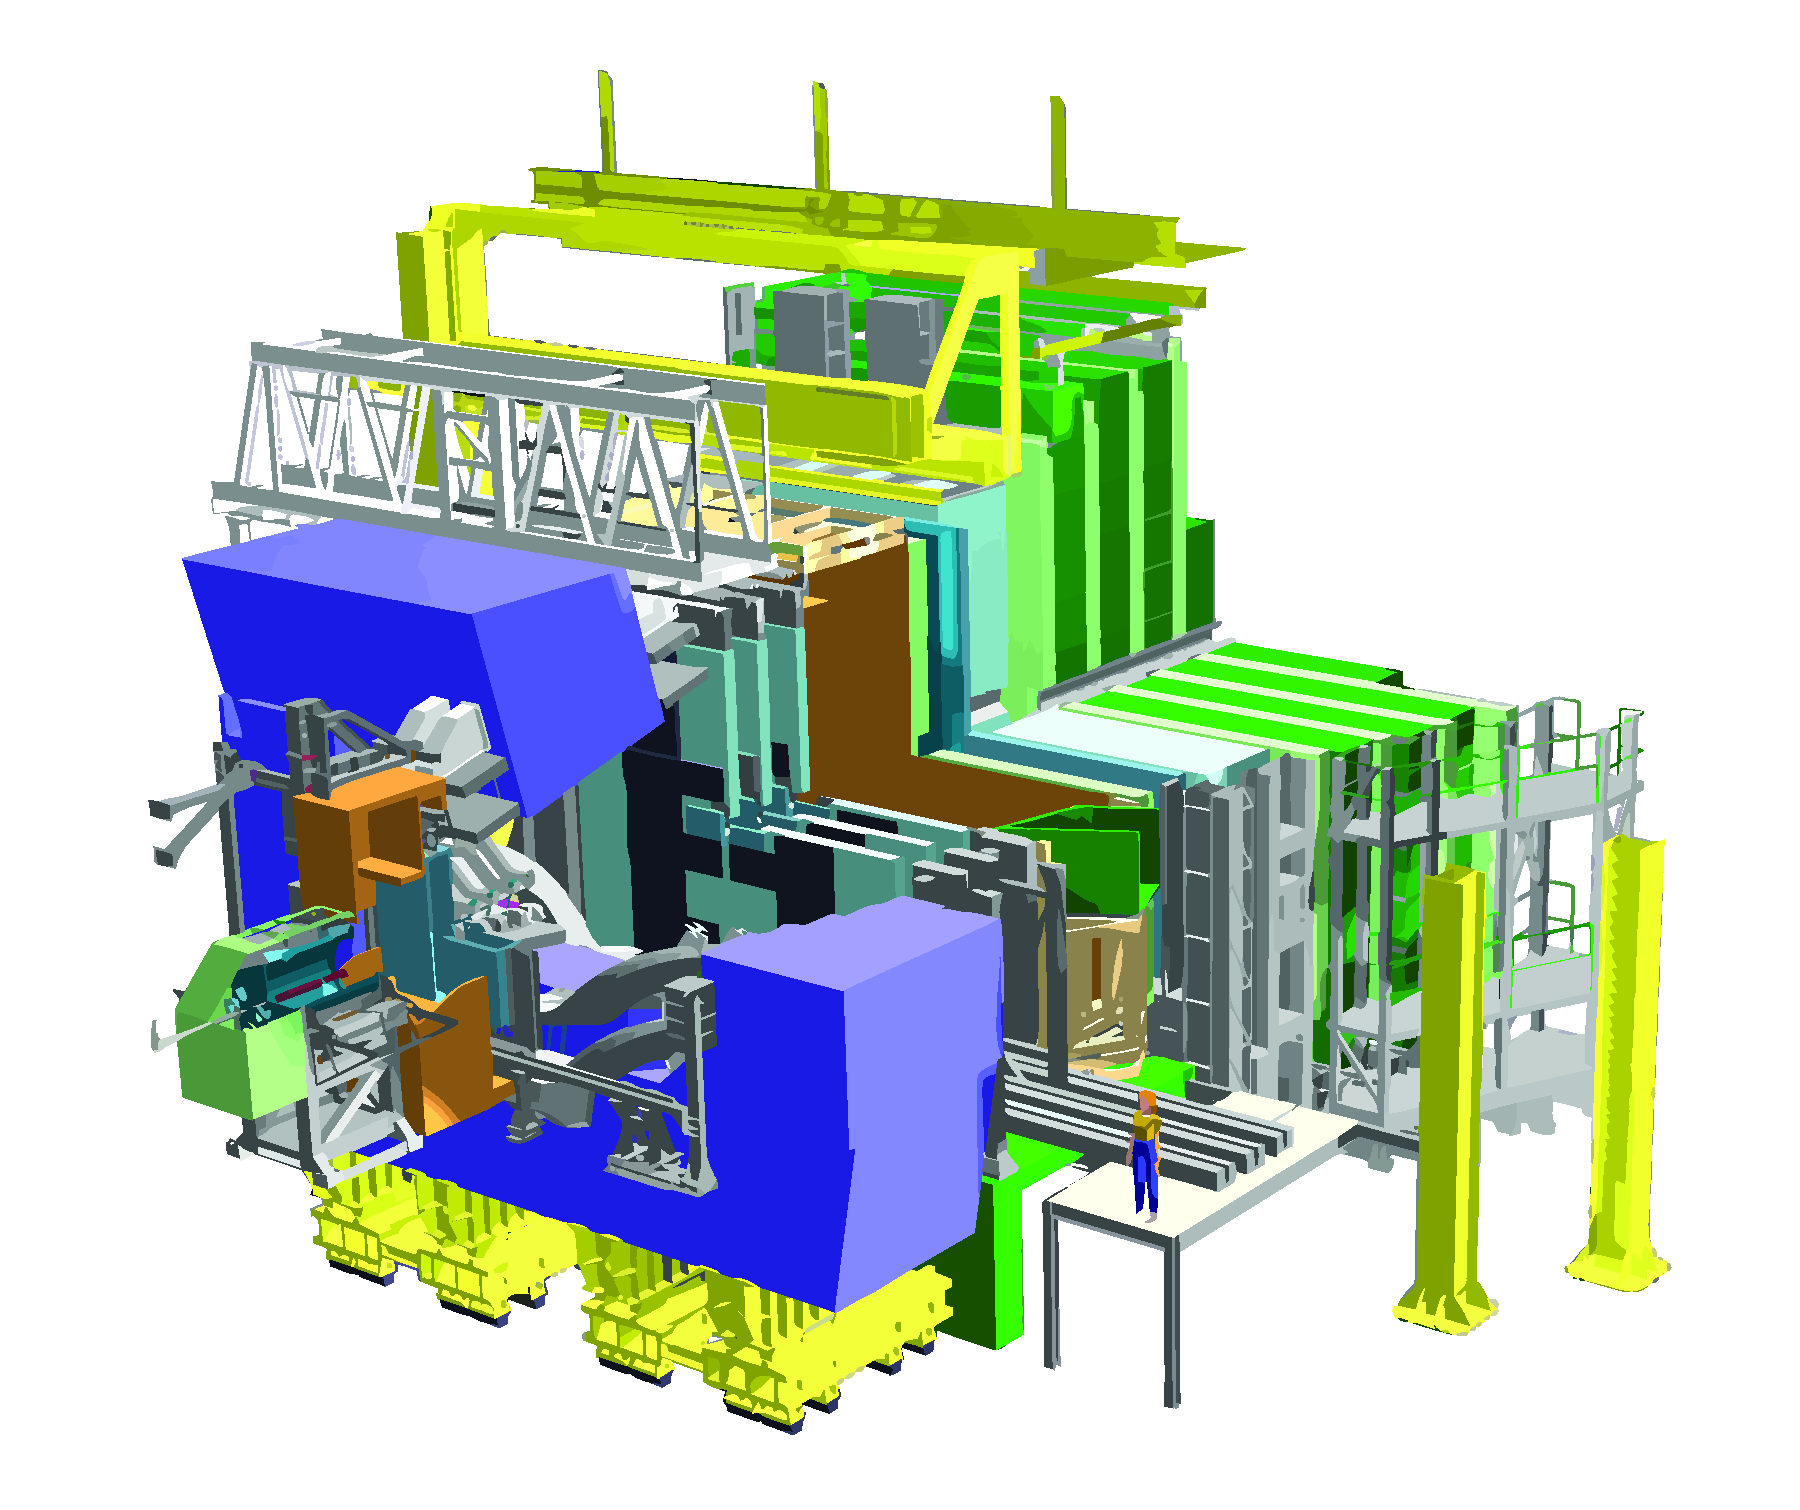
\includegraphics[width=0.48\textwidth]{LHCb.pdf}} \hfill
\caption{Esquemas (no en la misma escala) de los cuatro detectores principales de \lhc.} \label{fig_lhcdetect}
\end{figure}




%%%%%%%%%%%%%%%%%%%%%%%%%%%%%%%%%%%%%%%%%%%%%%%%%%%%%%%%%%%%%%%%%%%%%%%%%%%%%%%%
\section{El detector} %%%%%%%%%%%%%%%%%%%%%%%%%%%%%%%%%%%%%%%%%%%%%%%%%%%%%%%%%%

La idea original para la que \lhcb, Figura \ref{fig:partsLHCb}, fue diseñado era hacer estudios de precisión de los decaimientos raros de los cuarks \emph{charm} y, sobre todo, \emph{bottom} \cite{Adeva:1224241,Alves:1129809}. El experimento, de $4500$ toneladas, situado en la antigua caverna de DELPHI (\textit{Detector with Lepton, Photon and Hadron Identication}, uno de los cuatro principales experimentos de LEP), fue diseñado específicamente para filtrar estas partículas. %La propia decisión de centrarse en los mesones B (aquellos formados por un cuark b), provoca una constricción en el propio diseño del detector.  \color{norm}

\begin{figure}[H]
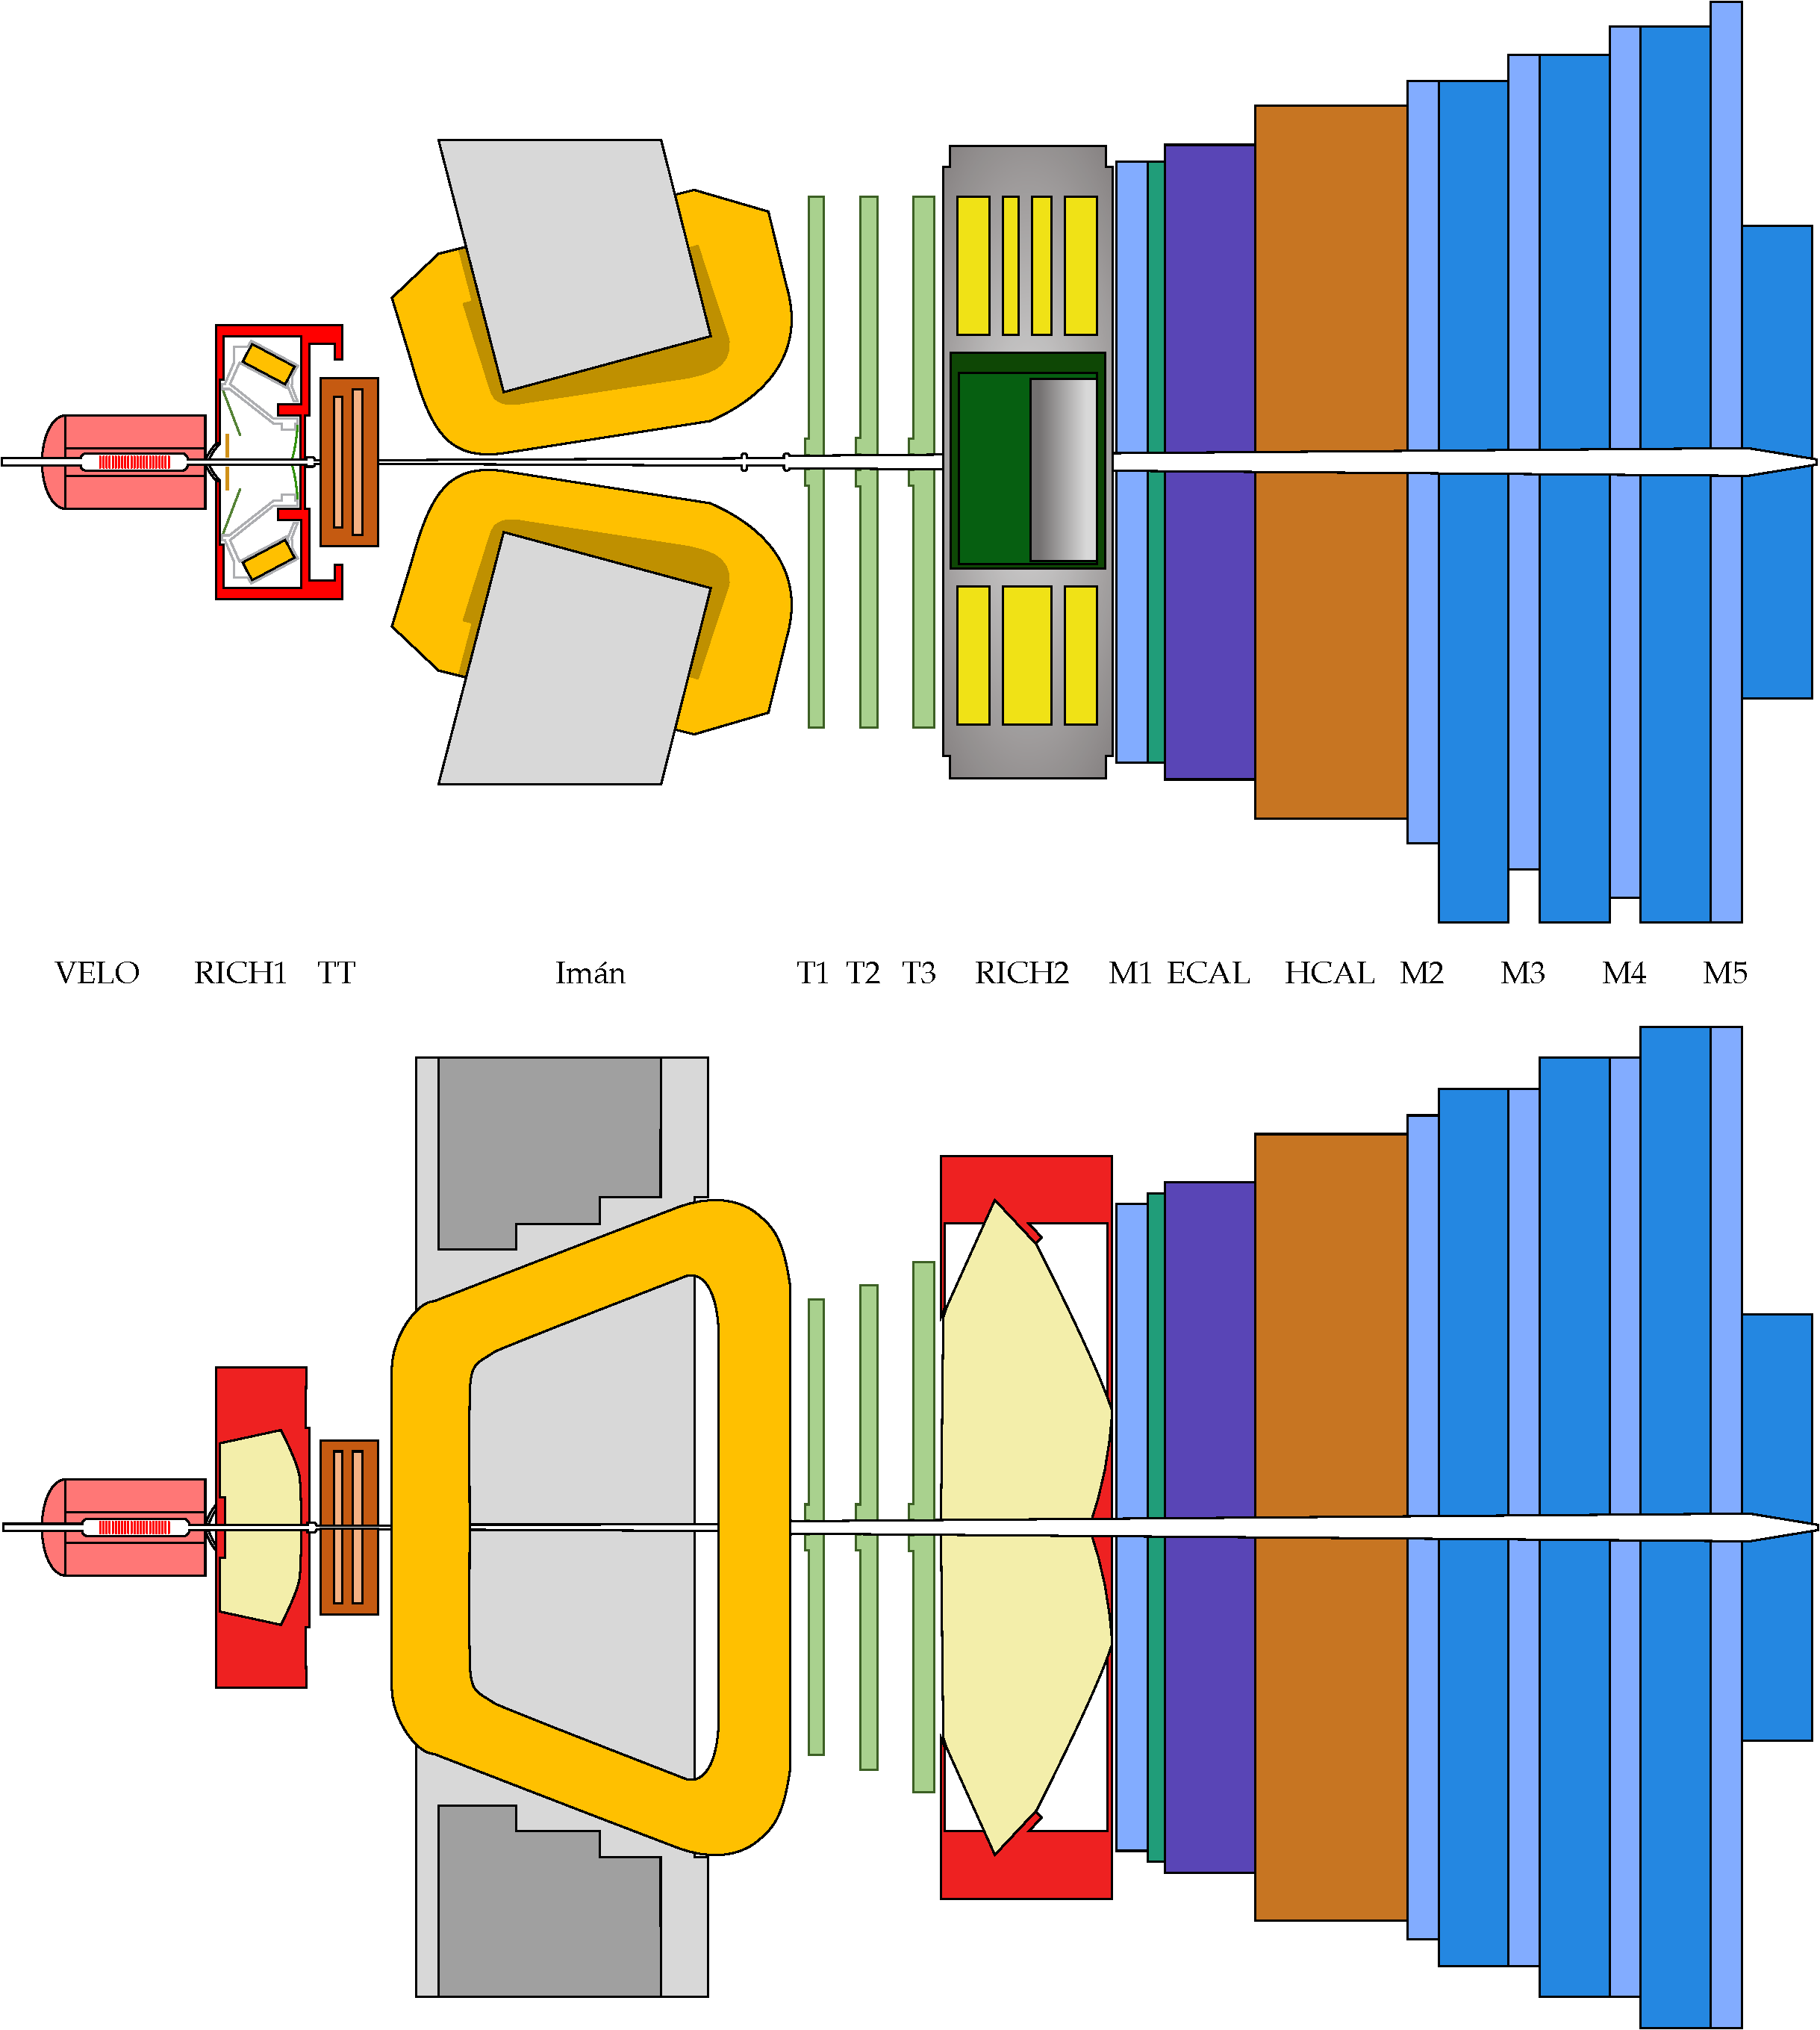
\includegraphics[width=\textwidth]{LHCbParts.pdf}
\caption{Detector \lhcb en dos vistas: arriba \textit{non-bending plane} (plano paralelo al campo magnético) y abajo \textit{bending plane} (plano perpendicular al campo magnético).}	\label{fig:partsLHCb}
\end{figure}

Dado que la sección eficaz de producción de pares $b$--$\bar b$ es muy alta para ángulos pequeños a estas energías 
%(ver figura <FIGURA>)
%  angle production figure
, \lhcb, a diferencia de los otros 3 detectores principales de LHC que tienen una estructura de barril y aceptancia quasi--$4 \pi$, es un detector de brazo único orientado en la dirección positiva \color{vero} de la circulación de los haces. \color{norm}
%
Así mismo, \lhcb se diseñó para trabajar a una luminosidad de entre $2$ y $5 \times 10^{32} \, \mathrm{cm^{-2}\, s^{-1}}$ \cite{Alves:1129809}, en vez de la nominal de \lhc $ 10^{34} \, \mathrm{cm^{-2}\, s^{-1}}$, de esta forma se puede asegurar una determinación precisa del vértice principal (PV) y del secundario (SV ---donde decaen las partículas) .

Su aceptancia varía desde los
 $10$ mrad hasta los $300$ mrad en el plano perpendicular al campo magnético ($250$ mrad en el paralelo) respecto al eje de los protones. Traduciendo estas cifras en pseudorapidez, $\eta$, \lhcb tiene una aceptancia que cubre el rango $2 < \eta < 5$ \cite{Alves:1129809}.

%TODO check footnote


%%%%%%%%%%%%%%%%%%%%%%%%%%%%%%%%%%%%%%%%%%%%%%%%%%%%%%%%%%%%%%%%%%%%%%%%%%%%%%%%
\subsection{Sistema de trazado} %%%%%%%%%%%%%%%%%%%%%%%%%%%%%%%%%%%%%%%%%%%%%%%%

A la hora de tomar los datos, \lhcb \cite{Alves:1129809} necesita tener una precisa determinación de las trayectorias en las que se desplazan las partículas.  Una vez que se reconstruye la traza, se puede determinar la carga de la partícula visto su comportamiento frente al imán, por ejemplo. Las combinaciones de varias trazas llevan a poder reconstruir vértices y medir con precisión su localización en el espacio. \lhcb cuenta con 3 sistemas de trazado: \color{vero} el \emph{Vertex Locator} (VELO), el \emph{Tracker Turicensis} (TT) y las estaciones de \emph{Tracking} 1, 2 y 3 (Tx). \color{norm}

\begin{figure}[H]
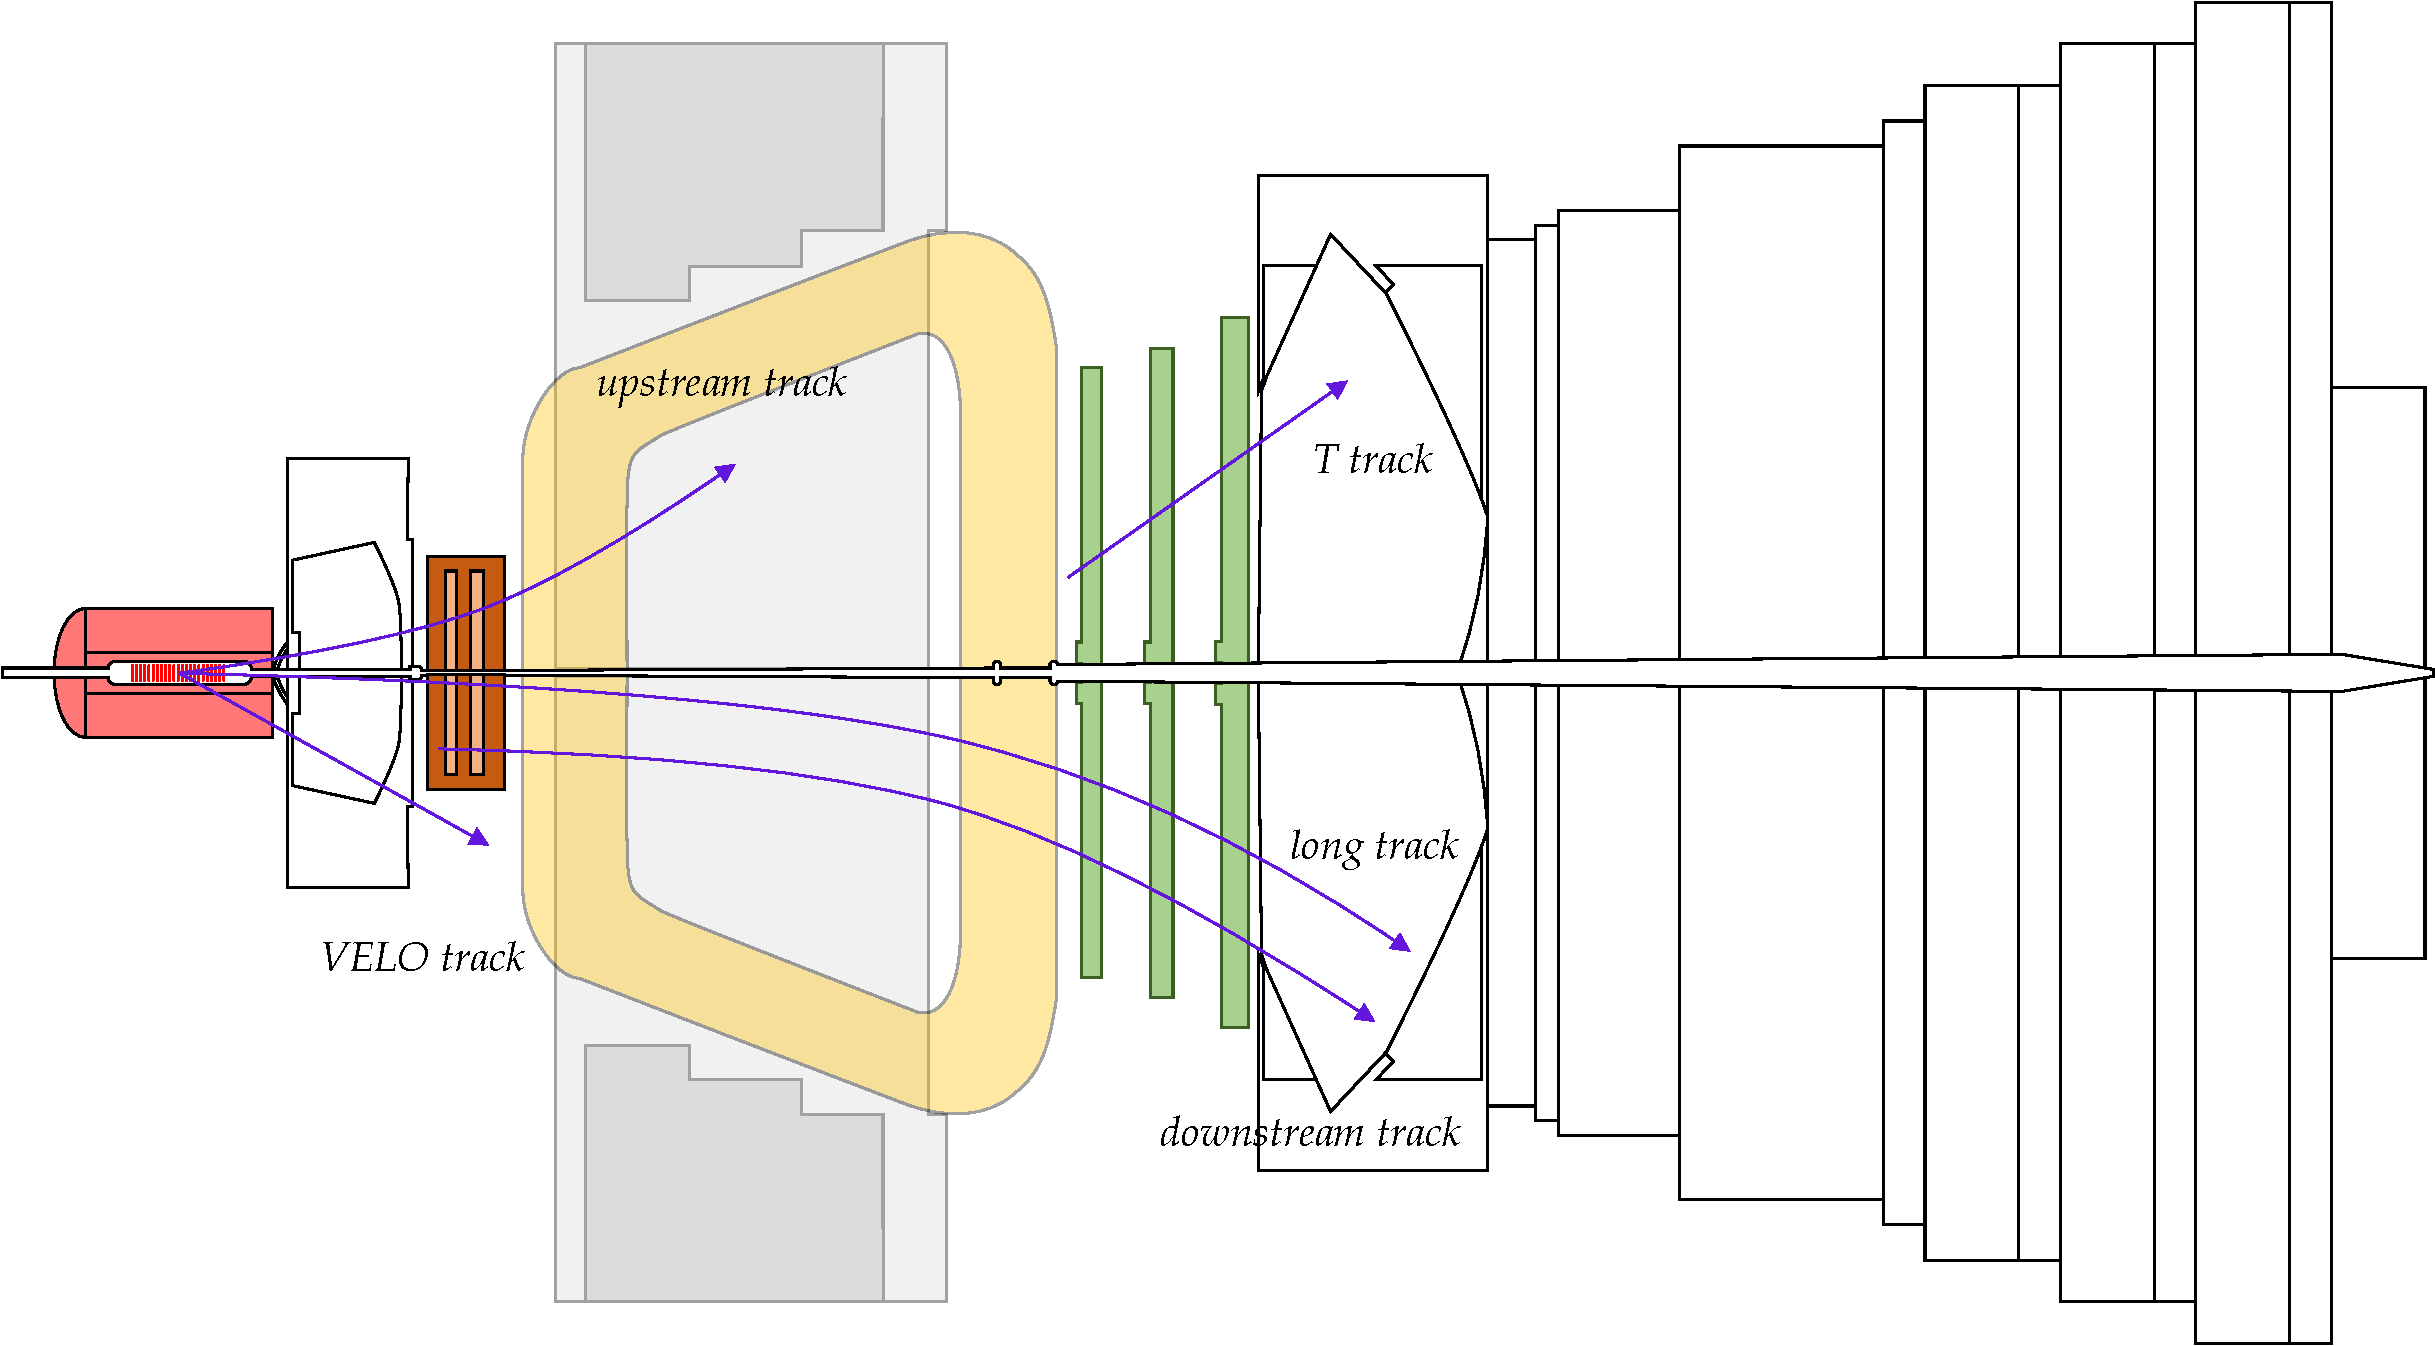
\includegraphics[width=\textwidth]{LHCbTracks}
\caption{Representación de los tipos de trazas, dependiendo de los volúmenes del espectrómetro que atraviesen.}	 \label{fig_tracks}
\end{figure}

\vspace*{-1cm}

La reconstrucción de eventos se fundamenta en determinar las trayectorias de todas las partículas cargadas y la posición en donde estas fueron generadas: los vértices. Para ello es preciso emplear, combinadamente, la información proporcionada por los tres sistemas de trazado. Dependiendo de la posición del vértice y de los \emph{hits},  se tienen las distintas posibilidades \color{vero} de la Figura \ref{fig_tracks}:\color{norm}
\begin{itemize}
	\item \textit{Long tracks}: Atraviesan todo el sistema de trazado, desde el VELO a las estaciones Tx y, dado que todos los detectores las miden, acaban siendo las medidas de momento más precisas, y las más importantes para \lhcb.
	\item \textit{Upstream tracks}: Atraviesan el VELO  y el TT; estos \emph{hits} se corresponden con partículas de poco momento y que el imán desvió fuera de la aceptancia del detector.
	\item \textit{Downstream tracks}: Atraviesan el TT y las estaciones Tx; estas trazas se corresponden con partículas de larga vida media que decaen fuera del VELO.
	\item \textit{VELO tracks}: Solo se miden en el detector homónimo y se corresponden con partículas que salen con un ángulo muy grande o hacia atrás, y que sirven principalmente en la reconstrucción del PV.
	\item \textit{T tracks}: Solo atraviesan las estaciones Tx; y corresponden a menudo con partículas generadas en interacciones secundarias.
\end{itemize}
%




\subsubsection{Vertex Locator}  %%%%%%%%%%%%%%%%%%%%%%%%%%%%%%%%%%%%%%%%%%%%%%%%

El Localizador de Vértice (VELO, \emph{\textsc{Ve}rtex \textsc{Lo}cator}) mide las posiciones espaciales de las trazas cerca del punto de colisión protón--protón, siendo así el primero de los detectores en entrar en acción. Esto permite separar el vértice principal (PV) del vértice secundario en donde estarían los hadrones con cuarks $b$ o $c$.
Está conformado por $21 \times 2$ semidiscos ordenados, como se ve en la Figura \ref{fig_velo}, en la dirección del \textit{beam pipe}. Estos discos semicirculares están compuestos de micropistas de silicio y tienen en una cara los sensores $R$ (\emph{radial strips}) y en la opuesta los sensores $\phi$ (\emph{azimutal strips}), determinando así las coordenadas cilíndricas del PV. 

\vspace*{-0.5cm}

\begin{figure}[H]
\centering
\subfloat[Representación de los discos del VELO cerrado, para un \emph{beam} estable.\label{fig_velo_a1}]{\phantom{olaolaola}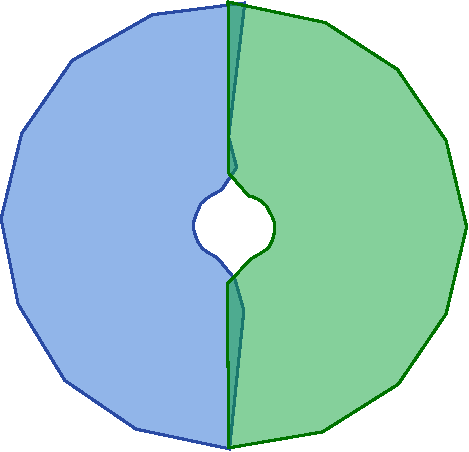
\includegraphics[height=0.2\textwidth]{VELOClosed.pdf} \phantom{olaolaola}} \hfill
\subfloat[Representación de los discos del VELO abierto, para la entrada de protones a \lhc.\label{fig_velo_a2}]{\phantom{olaol} 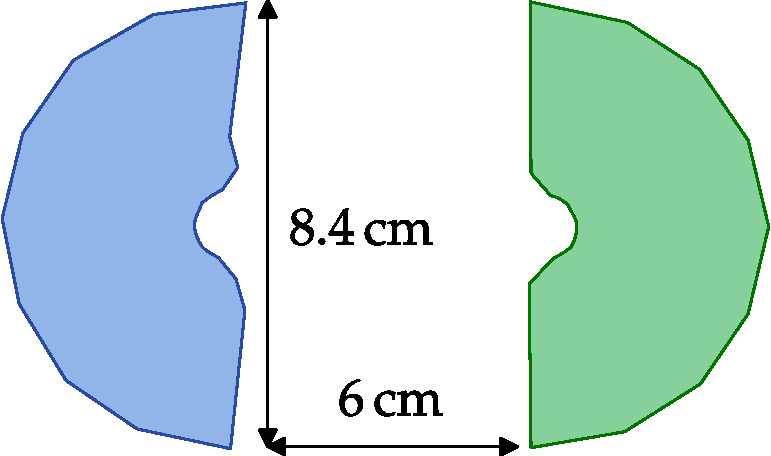
\includegraphics[height=0.2\textwidth]{VELOOpened.pdf} \phantom{olaol}}
 \\ 
 
\subfloat[Ubicación de los 42 semicírculos de micropistas de silicio que conforman el VELO. Se observa la alternancia entre detectores radiales y azimutales.\label{fig_velo_b}]{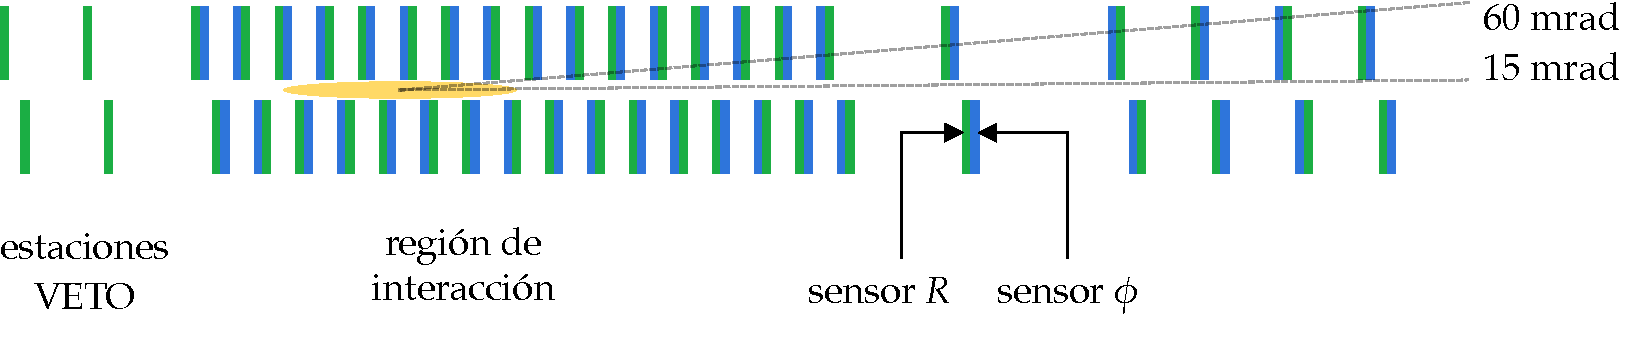
\includegraphics[width=\textwidth]{VELOStructure.pdf}} \hfill
\caption{Representación esquemática de partes del \emph{Vertex Locator}, detector donde se determina el PV y SV.} \label{fig_velo}
\end{figure}


Para tener la mejor precisión posible en la resolución del PV, la medida de la traza convendría que se realizase lo más cerca posible de la interacción. El VELO tiene área sensible desde tan solo $8$ mm del \emph{beam pipe}, demasiado pequeña para el proceso de inyección de protones al LHC. Cuando se están introduciendo protones en el tubo principal, o mientras hay inestabilidades en el haz, el VELO se puede separar $3$ cm del tubo, protegiendo así al detector de la radiación. El VELO es capaz de determinar las longitudes de decaimiento del B y D con una precisión de entre $220$ y $375 \,\upmu$m, y localizar el PV con una precisión de hasta $10 \, \upmu$m en el plano perpendicular y hasta $42 \,\upmu$m en la dirección del haz.
 
La aceptancia del VELO cubre $1.6<\eta<4.9$ para las partículas en el PV. Al principio del VELO (\emph{vid.} Figura \ref{fig_velo_a2}) se observan 2 capas de pistas tipo R, que constituyen el \emph{pile--up VETO system}, que desecha los eventos que cuentan con un número grande de vértices primarios (\emph{high multiplicity events}) de esto se informa el \texttt{L0--trigger} descrito en \S \ref{sec_l0trigger}. 





\subsubsection{Tracking Turicensis y estaciones de trazado} %%%%%%%%%%%%%%%%%%%%

Tanto a la entrada como a la salida se colocan detectores de trazas, para ver cómo afecta el imán a sus trayectorias. El TT junto con las estaciones Tx son los principales detectores a la hora de medir el momento de las trazas en \lhcb \cite{Alves:1129809}. Tenemos dos tipos de detectores aquí: los detectores de micropistas de silicio y las cámaras de deriva.

\begin{description}

	\item[Silicon Tracker] \color{vero} Se denomina Silicon Tracker (ST) al conjunto formado por el TT y la parte más cercana al \emph{beam pipe} de las estaciones Tx, el Inner Tracker (IT); ambos ellos empleando la tecnología de silicio, cuyos detectores aparecen en la Figura \ref{fig_sillicontracker1}. \color{norm}
	El ST está compuesto por cuatro capas de detectores: dos verticales (la primera y última) y dos que se encuentran giradas por $\pm 5\,{}^{\circ}$ en medio de las anteriores. La separación entre las pistas es de $20\, \mathrm{\upmu m}$, lo que se traduce \color{vero} en \color{norm} una resolución de $50\,\mathrm{\upmu m}$. El TT está diseñado para cubrir el rango de aceptancia del detector, mientras que el ST se encuentra principalmente alrededor del \emph{beam pipe} y solo constituye el $1.3 \, \%$ de las estaciones de trazado.
\begin{figure}[H]
\centering
\subfloat[Representación del \emph{Tracker Turicensis}.\label{fig_st_a}]{\phantom{olaola}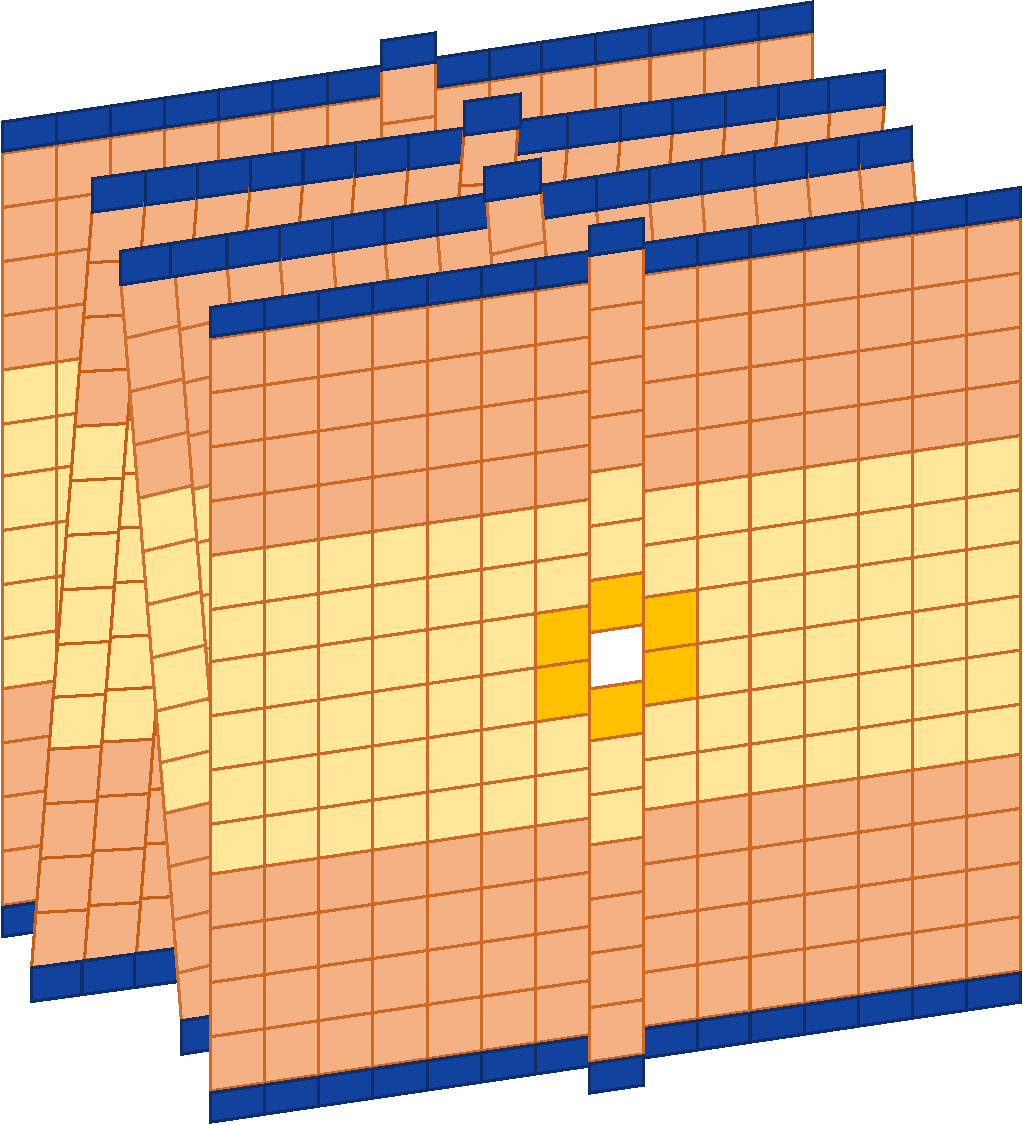
\includegraphics[width=0.3\textwidth]{TT.pdf}\phantom{olaola}} \hfill 
\subfloat[Representación de un \emph{Inner Tracker} de una estación Tx.\label{fig_st_b}]{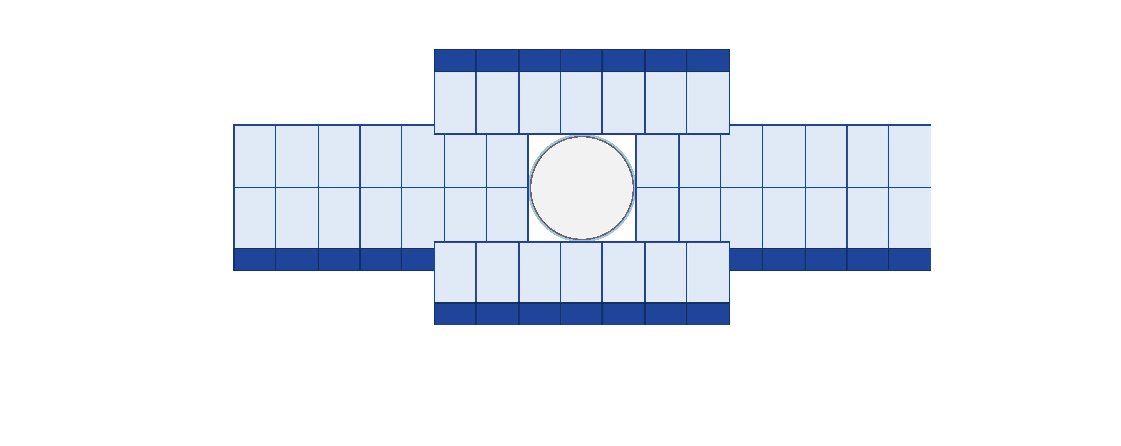
\includegraphics[width=0.5\textwidth]{IT.pdf}} \hfill
\caption{Elementos del \emph{Silicon Tracker}, las estaciones de trazado que emplean tecnología de silicio.} \label{fig_sillicontracker1}
\end{figure}

	\item[Outer Tracker]  Las \color{vero}estaciones Tx, representadas en la Figura \ref{fig_sillicontracker2}, \color{norm} se conforman en su parte más externa del OT, un detector de cámaras de deriva que tiene una resolución en la traza de $200\, \mathrm{\upmu m}$ y que emplea una mezcla 70--30 de argon y $\mathrm{CO_2}$ como gas. Los módulos del OT se organizan en tres estaciones de trazado, cada una de ellas con cuatro capas de detección que siguen el mismo patrón que las descritas para el ST.
\begin{figure}[H]
\centering
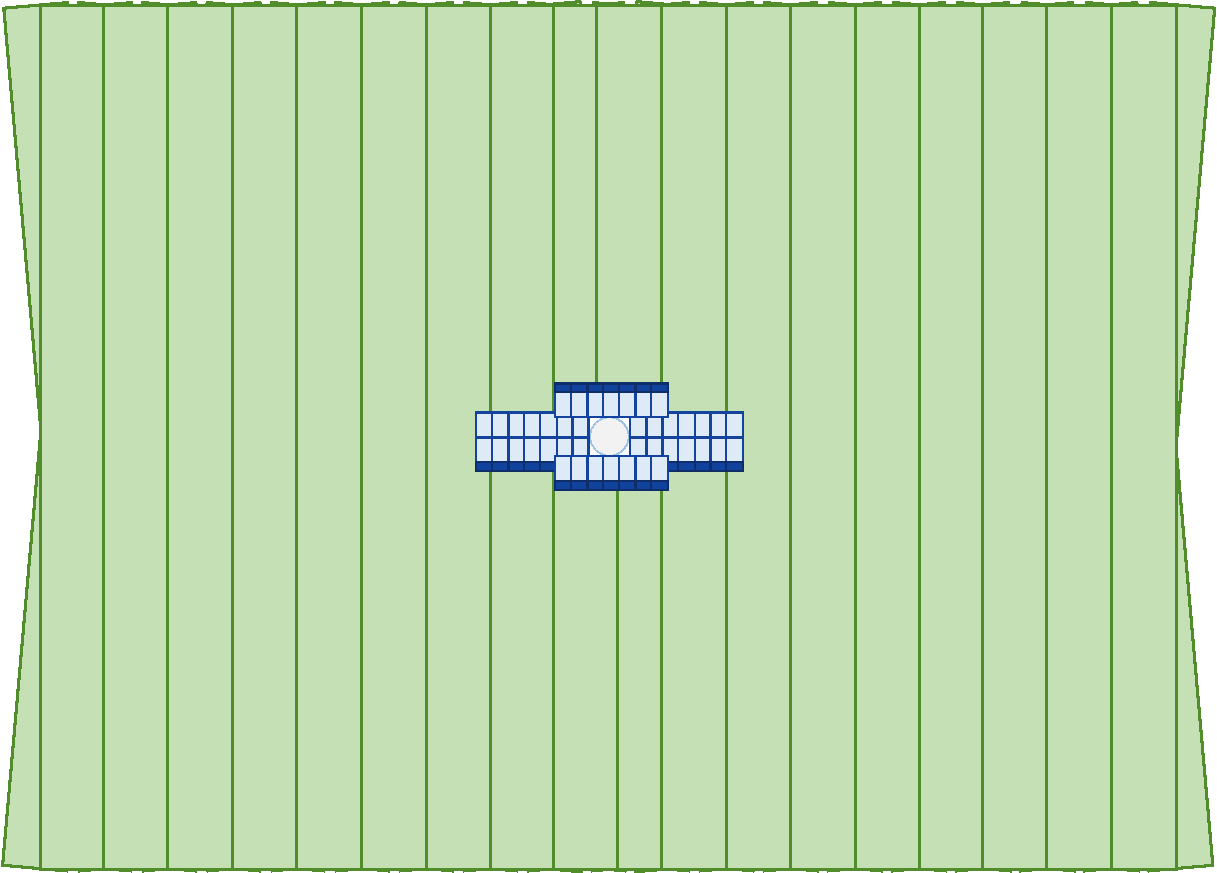
\includegraphics[width=0.48\textwidth]{OT.pdf}
\caption{Representación de las estaciones Tx, donde puede verse en verde el \emph{Outer Tracker}.} \label{fig_sillicontracker2}
\end{figure}

\end{description} 



%%%%%%%%%%%%%%%%%%%%%%%%%%%%%%%%%%%%%%%%%%%%%%%%%%%%%%%%%%%%%%%%%%%%%%%%%%%%%%%%
\subsubsection{Imán} %%%%%%%%%%%%%%%%%%%%%%%%%%%%%%%%%%%%%%%%%%%%%%%%%%%

%TODO <FIGURE> of magnet
Se trata de un imán dipolar de bobinas convencional de $4 \, \mathrm{T\,m}$ de inducción magnética integrada a temperatura ambiente. Las bobinas, con forma de silla cónica y situadas simétricamente, están fabricadas en Al--99.7, puro que rodea a un núcleo de hierro; pesando cada una de ellas 27 toneladas \cite{Alves:1129809}.

Las partículas cargadas se curvan al atravesar el campo magnético, permitiendo así medir su momento. La diferencia entre el gradiente de las trazas en el VELO y en las estaciones Tx es inversamente proporcional al momento de la partícula. 
Destacar que, para la reducción de uncertidumbres sistemáticas a causa de diferencias en la detección de partículas con cargas distintas, \color{norm} se cambia periódicamente la dirección del campo magnético.



%%%%%%%%%%%%%%%%%%%%%%%%%%%%%%%%%%%%%%%%%%%%%%%%%%%%%%%%%%%%%%%%%%%%%%%%%%%%%%%%
\subsection{Identificación de partículas en los detectores} %%%%%%%%%%%%%%%%%%%%

La identificación de partículas es clave en \lhcb por varias razones, entre las que destacan: el permitir identificar el sabor (\emph{flavour}) de los mesones B y la posibilidad de eliminar \color{vero} fondos \color{norm} que son similares a la señal. En \lhcb hay tres tipos de detectores: RICH, calorímetros y detectores de muones.

%\begin{figure}[H]
%\includegraphics[scale=0.48]{lhcbpid}
%\caption{Representación de los detectores involucrados en la identificación de partículas. <maybe remove this one>}	
%\end{figure}



\subsubsection{Detectores RICH} %%%%%%%%%%%%%%%%%%%%%%%%%%%%%%%%%%%%%%%%%%%%%%%%

Estos detectores tienen como principio de funcionamiento la radiación Cherenkov emitida por partículas relativistas cargadas que atraviesan un medio con una velocidad superior a la de la luz ($c$) en ese medio. Entonces, midiendo $\cos \theta_C = \sfrac{c}{vn}$ ($n$ es el índice de refracción del medio) y combinándola con el momento, se puede inferir la masa y por tanto el tipo de partícula.

En \lhcb hay dos detectores RICH \cite{Alves:1129809}, uno a la entrada y otro a la salida del imán dipolar. El RICH1, situado antes del imán, emplea aerogel y $\mathrm{C_4F_{10}}$ como radiadores y está optimizado para partículas de bajo momento, $1-60 \, \mathrm{GeV\, c^{-1}}$. EL RICH2, situado después de las estaciones de trazado Tx, emplea $\mathrm{CF_4}$ como radiador y detecta partículas con momento $15-100 \, \mathrm{GeV\, c^{-1}}$. Pueden verse representaciones de ambos detectores en la Figura \ref{fig_richdectectors}.
%
La aceptancia del RICH1 es de $250$ mrad, mientras que la del RICH2 es de $120$ mrad. En ambos, la luz Cherenkov que se produce al atravesar las partículas del material radiador se refleja en combinaciones de espejos planos y esféricos conduciéndola fuera de la aceptancia del detector donde es captada por \textit{Hybrid Photon Detectors} (HPD).

La misión fundamental del RICH es la identificación de partículas cargadas, nombradamente: $\uppi$, K y p.  Los anillos Cherenkov que se producen se identifican en los HPD  y se comparan con ciertas distribuciones para diferentes hipótesis en las trazas. Se define una \emph{likelihood} para todas las trazas y se minimiza para la hipótesis de partículas.

\begin{figure}[H]
\centering
\subfloat[Representación de la vista lateral del RICH1.\label{fig_rich1}]{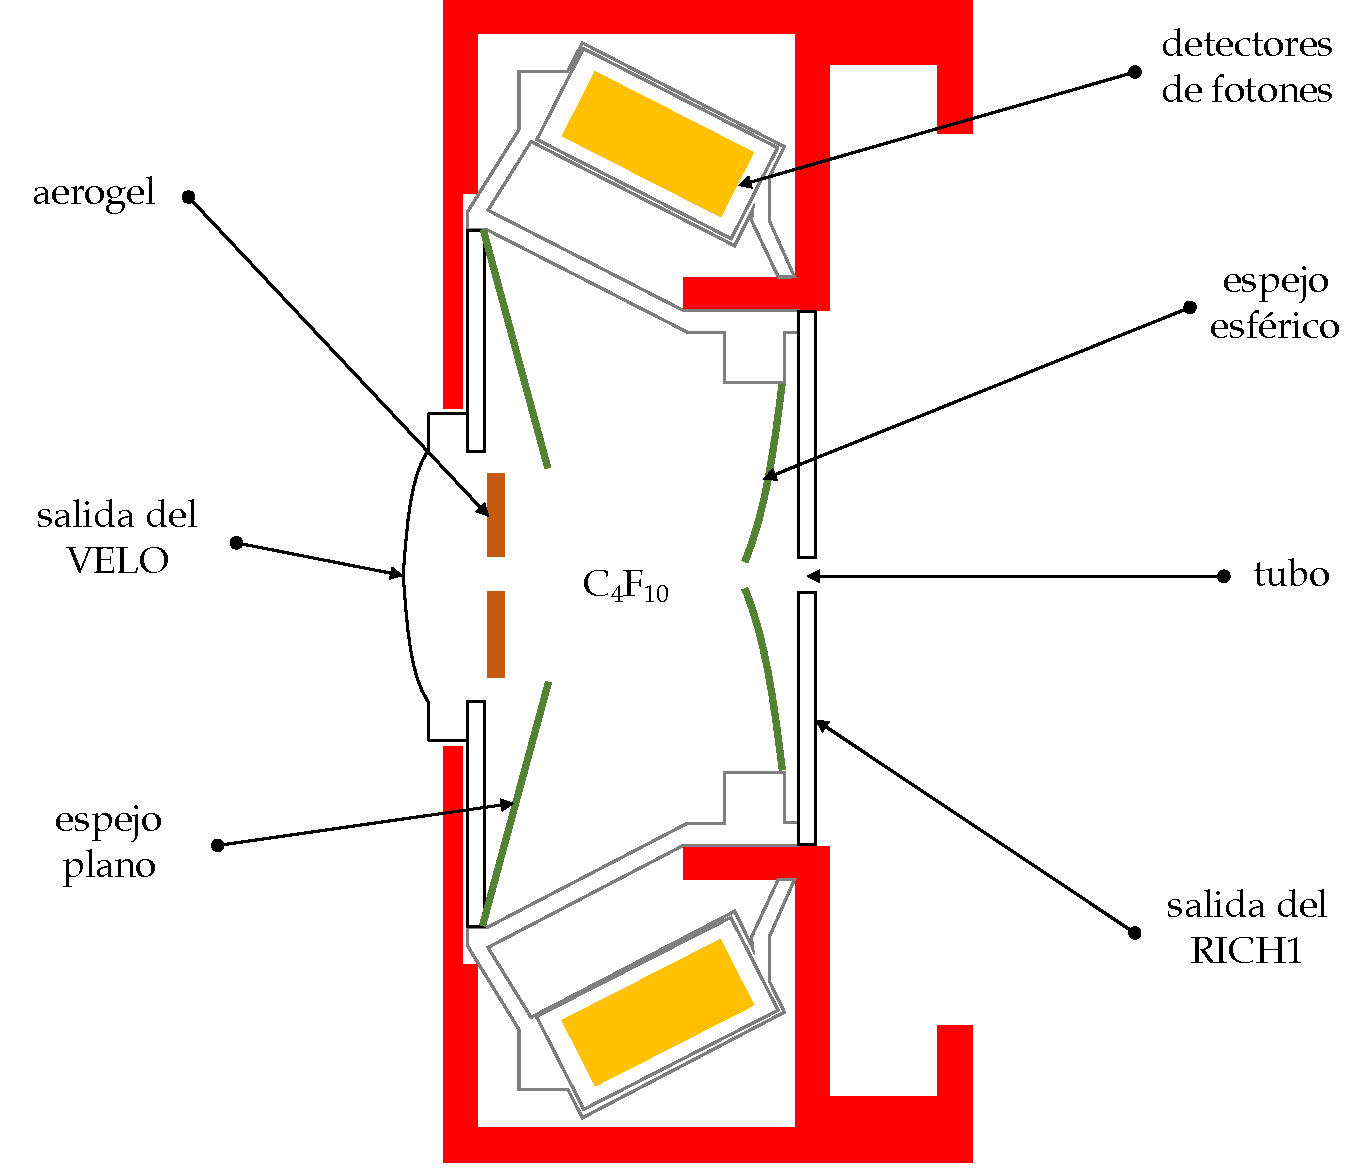
\includegraphics[height=0.4\textwidth]{RICH1}} \hfill
\subfloat[Representación de la vista desde arriba del RICH2.\label{fig_rich2}]{\phantom{olaola}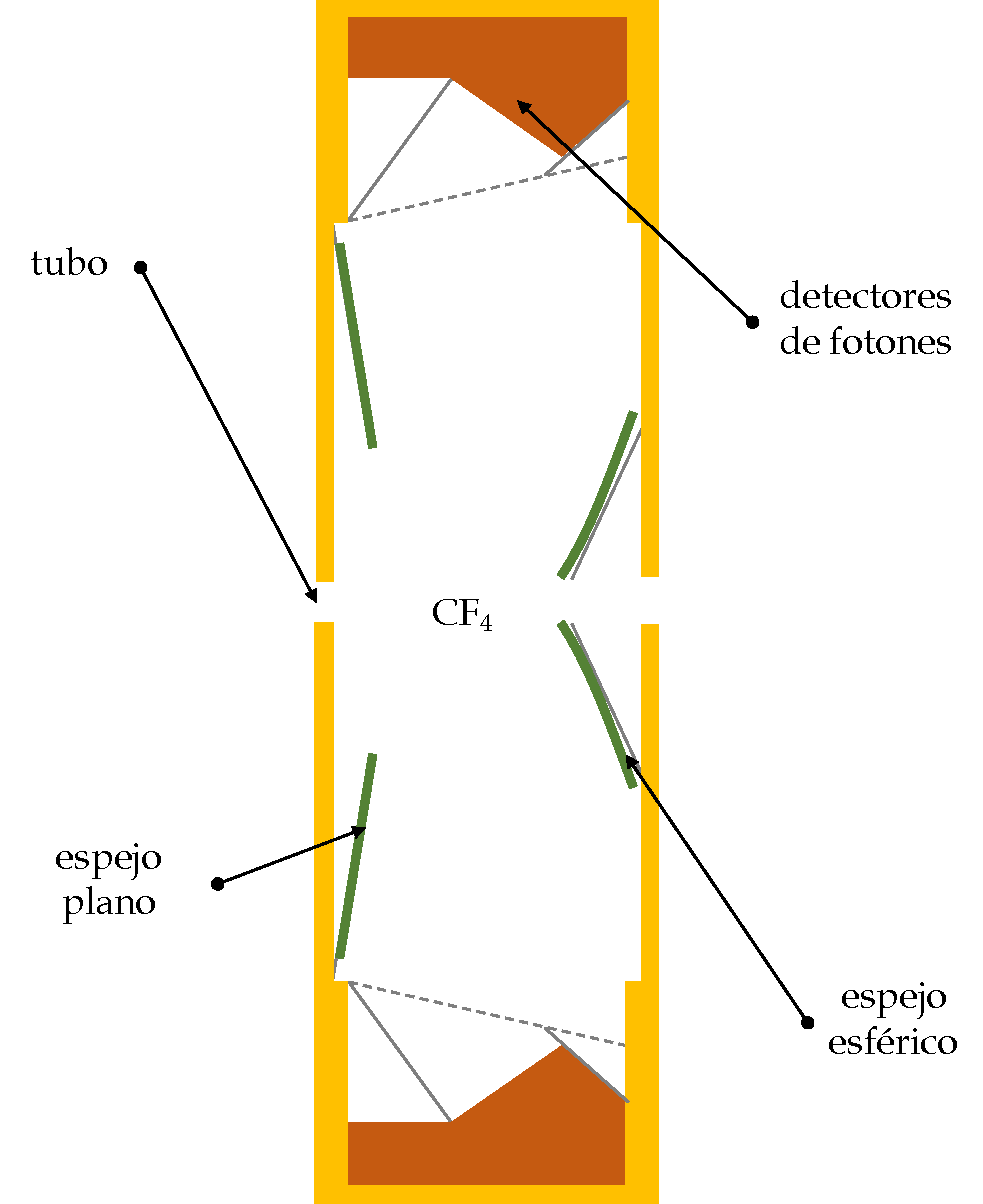
\includegraphics[height=0.4\textwidth]{RICH2}\phantom{olaola}} \hfill
\caption{Representación de los detectores RICH y de sus partes principales.} \label{fig_richdectectors}
\end{figure}



\subsubsection{Calorímetros} %%%%%%%%%%%%%%%%%%%%%%%%%%%%%%%%%%%%%%%%%%%%%%%%%%%

El sistema de calorímetros tiene como principal función determinar la energía \color{vero} transversal, \color{norm} $E_T$, que necesita el \texttt{L0}--\emph{trigger}, midiéndola a partir de la que depositan las partículas en las capas de material absorbente. 
Además, con la configuración de calorímetros de \lhcb, se pueden identificar también las partículas, una vez estas depositan toda su energía cinética dando lugar a cascadas de partículas que son caracterizadas por los calorímetros. Todos los calorímetros se encuentran divididos en celdas, permitiendo así medir la posición de la energía que se va depositando en las diferentes celdas.

%\begingroup
%\mySfFamily
%This should be sans-serif : $dfgd, \Q, \N, \Z, \C$ are sets.
%\endgroup


El sistema de calorímetros de \lhcb \cite{Alves:1129809} se compone de cuatro elementos, ordenadamente: \emph{Scintillating Pad Detector} (SPD), que detecta si las partículas entrantes son neutras o tienen carga; \emph{Preshower} (PS), que distingue entre electrones y hadrones cargados, y fotones de hadrones neutros, gracias a una lámina de plomo que se ubica entre el SPD y este mismo; \emph{Electromagnetic Calorimeter} (ECAL), que alterna centelleadores y láminas de plomo para identificar partículas no hadrónicas y tiene un espesor de 25 longitudes de radiación; \emph{Hadronic Calorimeter} (HCAL), que alternando material centelleador con láminas de hierro y con un espesor de 6 longitudes de interacción nuclear, identifica los hadrones.

\begin{figure}[H]
\centering
\subfloat[Representación de las celdas de un cuarto del ECAL.\label{fig_ecal}]{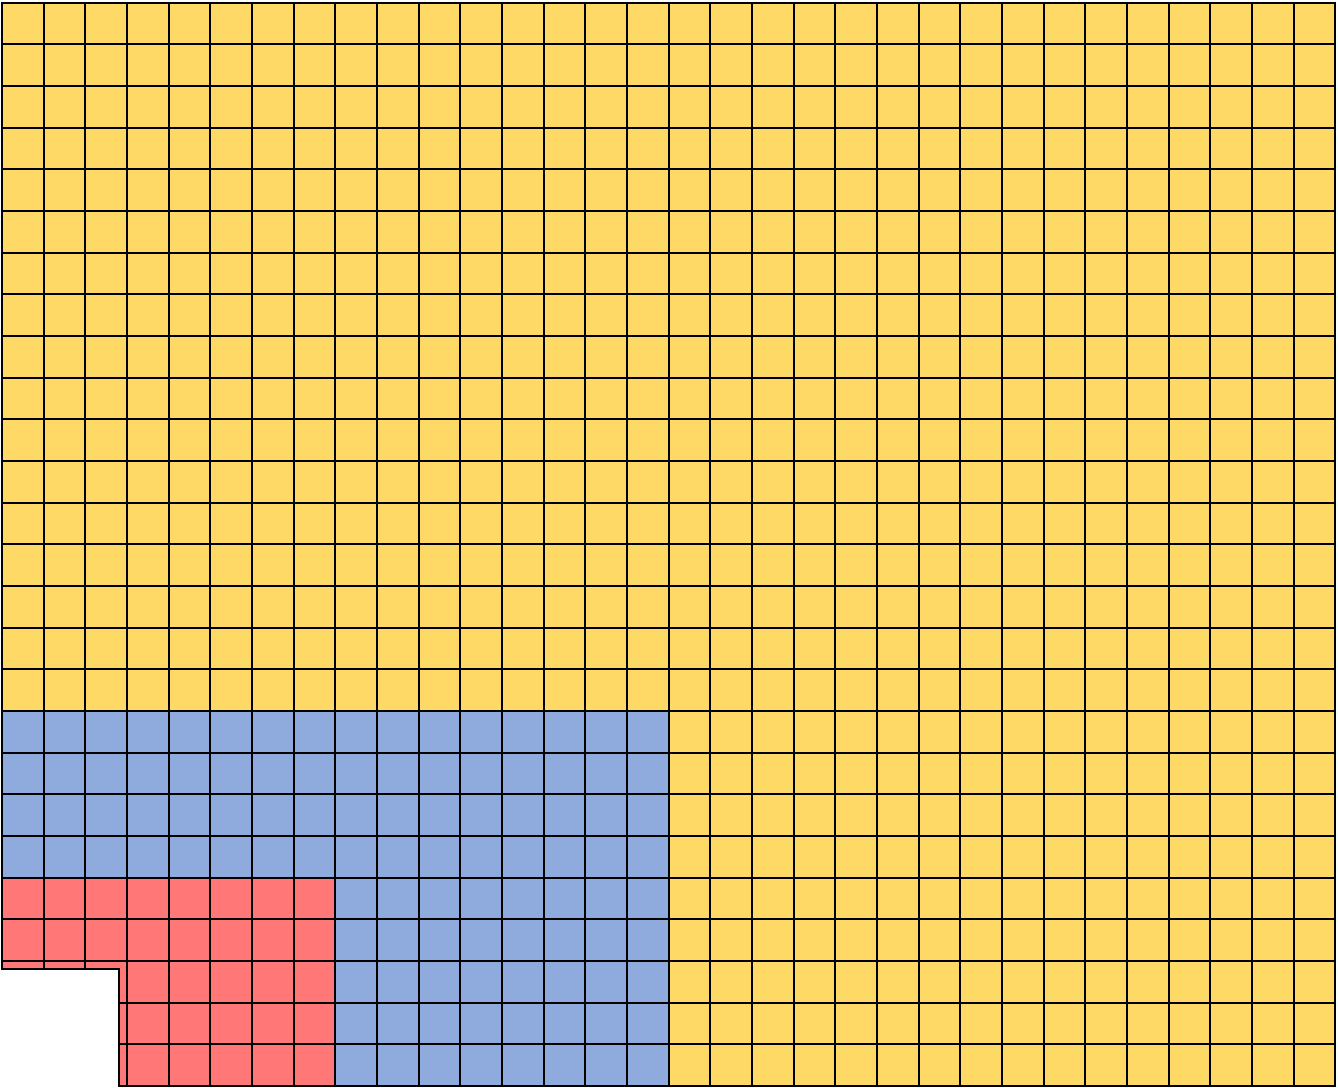
\includegraphics[width=0.48\textwidth]{ECAL}} \hfill
\subfloat[Representación de las celdas de un cuarto del HCAL.\label{fig_hcal}]{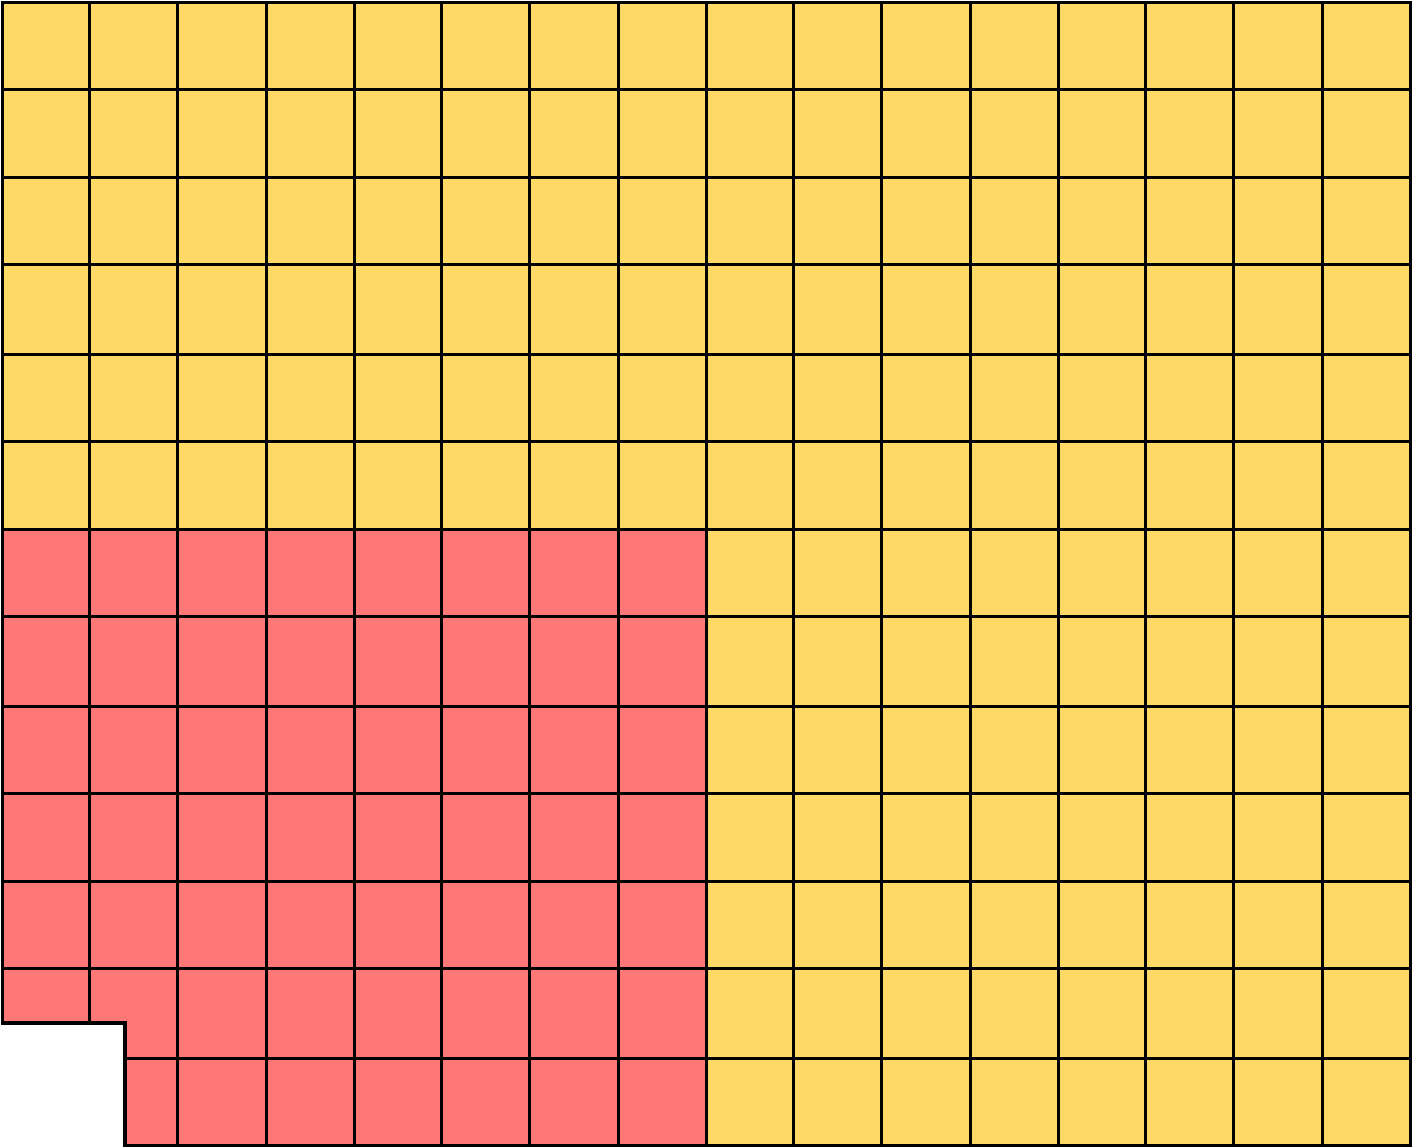
\includegraphics[width=0.48\textwidth]{HCAL}} \hfill
\caption{Representanciones gráficas de los calorímetros ECAL y HCAL.} \label{fig_calos}
\end{figure}

Tanto el ECAL como el HCAL, que pueden verse en la Figura \ref{fig_calos}, emplean el mismo principio de detección: captar centelleos de las partículas cargadas y transmitir estos fotones vía fibras de onda a tubos fotomultiplicadores. 
%
En el momento de identificar las partículas, el calorímetro provee al \texttt{L0} información combinada de ECAL, PS y SPD que permite la identifiación de partículas: el \texttt{CALO PID}.
%
Al igual que el RICH, se hacen tests para discriminar las partículas mediante medias de log--\emph{likelihood} calculadas con las deposiciones de energía en las distintas posiciones de los calorímetros.

%TRIGGER search triger and make it italic

\subsubsection{Sistema de muones} %%%%%%%%%%%%%%%%%%%%%%%%%%%%%%%%%%%%%%%%%%%%%%

Los muones son partículas muy penetrantes debido a su poca sección eficaz de interacción, y por ello pueden atravesar los calorímetros sin apenas perder más que una pequeña energía, pudiendo así detectarse al final de \lhcb, en las cámaras de muones. \color{new} El sistema de muones es empleado tanto en el \texttt{L0}--trigger, para seleccionar muones con un alto momento tranverso; y en la reconstrucción offline, para identificarlos. \color{norm}

El sistema de muones de \lhcb \cite{Alves:1129809} se compone de 5 estaciones, M1--M5: M1 se sitúa entre el RICH2 y el SPD, y usa tecnología de \emph{Gas Electron Multiplier} (GEM) puesto que en esta región hay una mayor tasa de partículas; las cámaras M2-M5 se encuentran después del HCAL y emplean \emph{Multiwire Proportional Chambers} (MWPC) \color{new} separados por $80$ cm de hierro. La aceptancia general del sistema de muones está entre $20 (16)$ mrad y $306 (258)$ mrad en el plano perpendicular (paralelo) al campo magnético. \color{norm}

\begin{figure}[H]
\centering
\includegraphics[width=0.6\textwidth]{MuonChamber.pdf}
\caption{Representación de un cuarto de la cámara de muones M1, en donde se pueden apreciar los \emph{pads} y las celdas detectoras. En cada región de las estaciones M2 y M3 (M4 y M5) el número de columnas detectoras de cada \emph{pad} es el doble (la mitad), manteniéndose constante el número de filas.}	\label{fig_muonchambers}
\end{figure}

La geometría de las diferentes estaciones varía el número de celdas detectoras en cada una, existiendo para cada estación zonas más y menos densas, tal y como puede apreciarse en la Figura \ref{fig_muonchambers}, acabando finalmente por computar un flujo similar en todas ellas.



%%%%%%%%%%%%%%%%%%%%%%%%%%%%%%%%%%%%%%%%%%%%%%%%%%%%%%%%%%%%%%%%%%%%%%%%%%%%%%%%

%TODO search fisica and change uppercase

%%%%%%%%%%%%%%%%%%%%%%%%%%%%%%%%%%%%%%%%%%%%%%%%%%%%%%%%%%%%%%%%%%%%%%%%%%%%%%%%
%%%%%%%%%%%%%%%%%%%%%%%%%%%%%%%%%%%%%%%%%%%%%%%%%%%%%%%%%%%%%%%%%%%%%%%%%%%%%%%%
\section{Sistema de trigger} %%%%%%%%%%%%%%%%%%%%%%%%%%%%%%%%%%%%%%%%%%%%%%%%%%%
%%%%%%%%%%%%%%%%%%%%%%%%%%%%%%%%%%%%%%%%%%%%%%%%%%%%%%%%%%%%%%%%%%%%%%%%%%%%%%%%
%%%%%%%%%%%%%%%%%%%%%%%%%%%%%%%%%%%%%%%%%%%%%%%%%%%%%%%%%%%%%%%%%%%%%%%%%%%%%%%%

\begin{wrapfigure}{r}{0.45\textwidth}
  \centering
  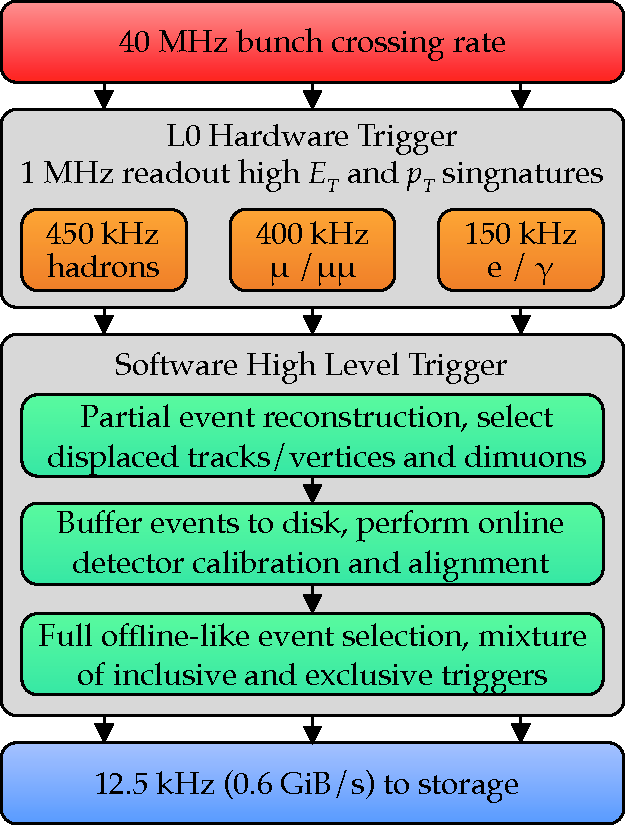
\includegraphics[width=0.4\textwidth]{Trigger.pdf}
  \caption{Esquema de actuación del \emph{trigger} de \lhcb en 2015.}	
\end{wrapfigure}

La frecuencia de colisión de \lhcb es de $40 \, \mathrm{M Hz}$, lo que se traduce en unos $10 \, \mathrm{M Hz}$ de eventos que entran en la aceptancia del detector. El número de \color{vero} eventos \color{norm} que puede ser grabado está limitado por la capacidad de cálculo \emph{offline}, de aproximadamente $2 \, \mathrm{k Hz}$, por lo que la cantidad de datos generada en  las colisiones de \lhc es demasiado alta para ser guardada directamente, y es por ello que se necesita de un eficaz sistema de \emph{trigger} que permita reducirla sin perder los eventos de mayor importancia para la Física. \color{new}
La estrategia principal del trigger se fundamenta en dos signaturas de las desintegraciones de los mesones B: la gran masa del B crea productos de desintegración con alto momento transverso $p_T$, y la larga vida media del B  genera productos con un parámetro de impacto grande respecto del vértice primario. \color{norm}
El sistema de trigger de \lhcb consta de dos niveles: \color{new} el Level--0 trigger (\texttt{L0}) de tipo hardware y el High Level Trigger (\texttt{HLT}) de tipo software \cite{Head_2014}. \color{norm}


%%%%%%%%%%%%%%%%%%%%%%%%%%%%%%%%%%%%%%%%%%%%%%%%%%%%%%%%%%%%%%%%%%%%%%%%%%%%%%%%
\subsection{Hardware trigger} %%%%%%%%%%%%%%%%%%%%%%%%%%%%%%%%%%%%%%%%%%%%%%%%%%
\label{sec_l0trigger}

La función del \texttt{L0} es reducir la tasa de datos a $1\,\mathrm{MHz}$, tasa a partir de la cual el detector se puede leer completamente. La decisión de si se debe o no aceptar el evento la toma la \textit{Decision Unit} (DU), basada en la información que síncronamente se está viendo en el detector a $40\,\mathrm{MHz}$. Para ello se usa la información siguiente:
\begin{itemize}
  \item \texttt{L0Calo}: Se toma la energía transversa de los \textit{clusters} que se producen en el calorímetro por los electrones, fotones, piones neutros y hadrones cargados. %esta se calcula en célus $2\times2$ .....
  \item \texttt{L0Muon}:  Se toma el momento transverso, $p_T$, de los muones o dimuones, llevándose a cabo una reconstrucción rápida de los candidatos con una resolución del $20 \, \%$. La DU solo hará uso de los dos candidatos con el $p_T$ más alto.
  \item Multiplicidades en el SPD: El número total de celdas del detector SPD que tienen un \textit{hit} se usa para obtener la multiplicidad de carga de la traza y rechazar así los eventos con un número muy alto de multiplicidades, que saturaría al \texttt{HLT} en la siguiente etapa.
\end{itemize}
%
Toda esta información se transmite a la \texttt{L0}DU, y se traduce con la calibración y triggers aleatorios en una decisión con una latencia máxima de $1 \, \mathrm{\upmu s}$. La decisión se envía a la electrónica \emph{front--end}, y si es positiva la electrónica de los detectores toma los datos y los envía a la EFF.



%%%%%%%%%%%%%%%%%%%%%%%%%%%%%%%%%%%%%%%%%%%%%%%%%%%%%%%%%%%%%%%%%%%%%%%%%%%%%%%%
\subsection{Software Trigger} %%%%%%%%%%%%%%%%%%%%%%%%%%%%%%%%%%%%%%%%%%%%%%%%%%
\label{sec_hltrigger}

Los datos aceptados por el \texttt{L0} se transmiten a la EFF, donde se ejecuta el \texttt{HLT}. El \texttt{HLT} es una aplicación \texttt{C++} que corre en cada CPU de la EFF y reduce la tasa de datos de 1 MHz hasta 12.5 kHz (en 2015). El \texttt{HLT} realiza una reconstrucción total de las trazas usando información \color{vero} de \color{norm} todo el detector, buscando discriminar la señal del ruido. \color{vero} Opera en dos \color{norm} partes:

\begin{itemize}
  \item \texttt{HLT1}: Usa información del VELO y las estaciones de trazado para reconstruir la traza 3D de la partículas y obtener el PV. Además se realiza una reconstrucción rápida de las trazas en las cámaras de muones, y se hace uso del parámetro de impacto, el momento total y transverso así como las deposiciones de energía en los calorímetros para reducir todavía más la tasa de datos.
  \item \texttt{HLT2}: A este nivel se puede reconstruir  totalmente el evento; se alcanzan los $12.5$ kHz que se graban para su posterior análisis, con una tasa de almacenamiento de $0.6 \, \mathrm{GiB s^{-1}}$.
\end{itemize}

\color{dieg}
El \texttt{HLT} funciona con las denominadas \emph{trigger lines}: cortes y criterios de selección similares a los aplicados durante los análisis. La implementación de las mismas puede ser bastante general o ceñirse a características más específicas. Por ejemplo, una línea de trigger puede exigir la presencia de dos muones, formando un vértice con una masa invariante en la ventana de masa de $\Jpsi$. \color{norm}

 \todo[inline]{meter líneas de jpsikk.}
 

Concretamente para el canal aquí estudiado, $\Bs \to \Jpsi \antikaon\kaon$, se aceptan todos los eventos que superen los criterios del \texttt{L0}. En  lo que al \texttt{HLT} concierne, existen dos categorías \cite{paperPhis}:
\begin{itemize}
  \item \texttt{Unbiased}: Se exige la correcta identificación de dos muones de carga opuesta con masa invariante mayor de $2700 \,\mathrm{MeV/}c^2$. La aceptancia en esta categoría es prácticamente constante, como puede verse en \S \ref{REF}.
  \item \texttt{Biased}: Se aceptan eventos si existe al menos un muón con momento transverso mayor de $1 \mathrm{GeV/}c$, y con un parámetro de impacto significativo respecto de los demás vértices primarios de ese evento; o bien, si se pasa la selección de un algoritmo multivariado que  identifica trazas de dos partículas, con un vértice secundario de suma de momento transverso alto y significativamente separado del vértice primario.
\end{itemize}

%%%%%%%%%%%%%%%%%%%%%%%%%%%%%%%%%%%%%%%%%%%%%%%%%%%%%%%%%%%%%%%%%%%%%%%%%%%%%%%%



%%%%%%%%%%%%%%%%%%%%%%%%%%%%%%%%%%%%%%%%%%%%%%%%%%%%%%%%%%%%%%%%%%%%%%%%%%%%%%%%
%%%%%%%%%%%%%%%%%%%%%%%%%%%%%%%%%%%%%%%%%%%%%%%%%%%%%%%%%%%%%%%%%%%%%%%%%%%%%%%%
%%%%%%%%%%%%%%%%%%%%%%%%%%%%%%%%%%%%%%%%%%%%%%%%%%%%%%%%%%%%%%%%%%%%%%%%%%%%%%%%